% !TEX root = ../main.tex
% !TeX spellcheck = en-US

\chapter{Results}
\label{cha:Results}
\subsection{Hydrodynamic Regime}
In search for a reduced model of the BGK equation, a first reduction and analysis of the provided data in the hydrodynamic regime is conducted. The error over the $L_2$-Norm derived from \cref{L2-Norm} assigns a value to each reduction algorithm enabling a evaluation.
\begin{table}[!htbp]\centering
	\begin{tabular}{ |c c| }
		\hline
		Algorithm & $L_2$ \\[.5ex]
		\hline
		SVD & 0.03  \\ 
		Fully Connected Autoencoder & 0.002 \\ 
		Convolutional Autoencoder & 0.02 \\ \hline
		\hline
	\end{tabular}
	\caption{L2-Error over Batch-Size}
	\label{Tab:Batch}
\end{table}
Furthermore the conservation quantities given in \cref{moment1} to \cref{moment3} of the prediction are analysed over the time average of each quantity. This normalization is given in \cref{Eq:Norm_Con_quantity}, where $\hat{\sigma}$ represents the given quantity.  
With more than $99\%$ of the total cumultative energy $S_N$ of the first five singular values calculated with \cref{Eq:cumsum} the SVD provides an upper bound to the number of intrinsic features the autoencoder should extract. \Cref{Fig:cumu_sing} shows the singular values (left) and the cumulative energy (right).
\begin{equation}
S_N = \sum_{k=1}^{N}a_k \qquad\textrm{with a sequence} \qquad\{a_k\}_{k=1}^{n} 
\label{Eq:cumsum}
\end{equation}  
\begin{figure}[!htbp]
	\centering
	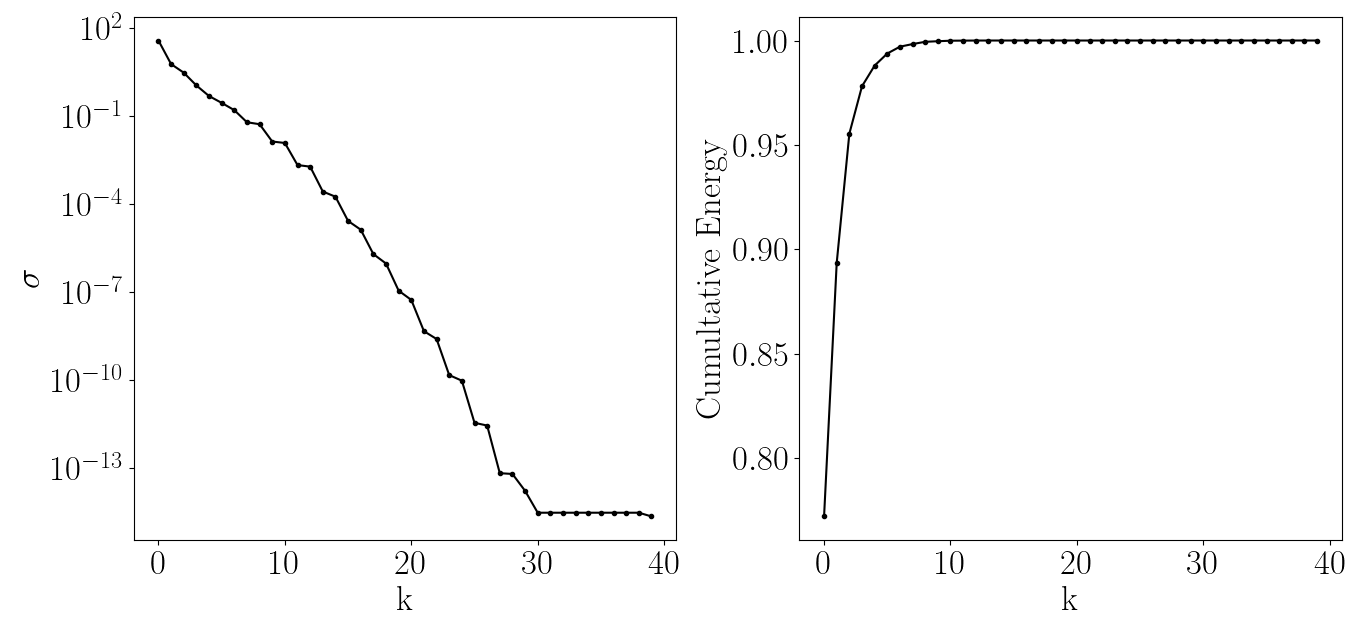
\includegraphics[width=\textwidth]{Figures/Cumultative_Singular_Values_kn001.png}
	\caption{Singular Values (left) and cumultative enrgy (right) over the number of singular values}
	\label{Fig:cumu_sing}
\end{figure}

\begin{figure}[!htbp]
	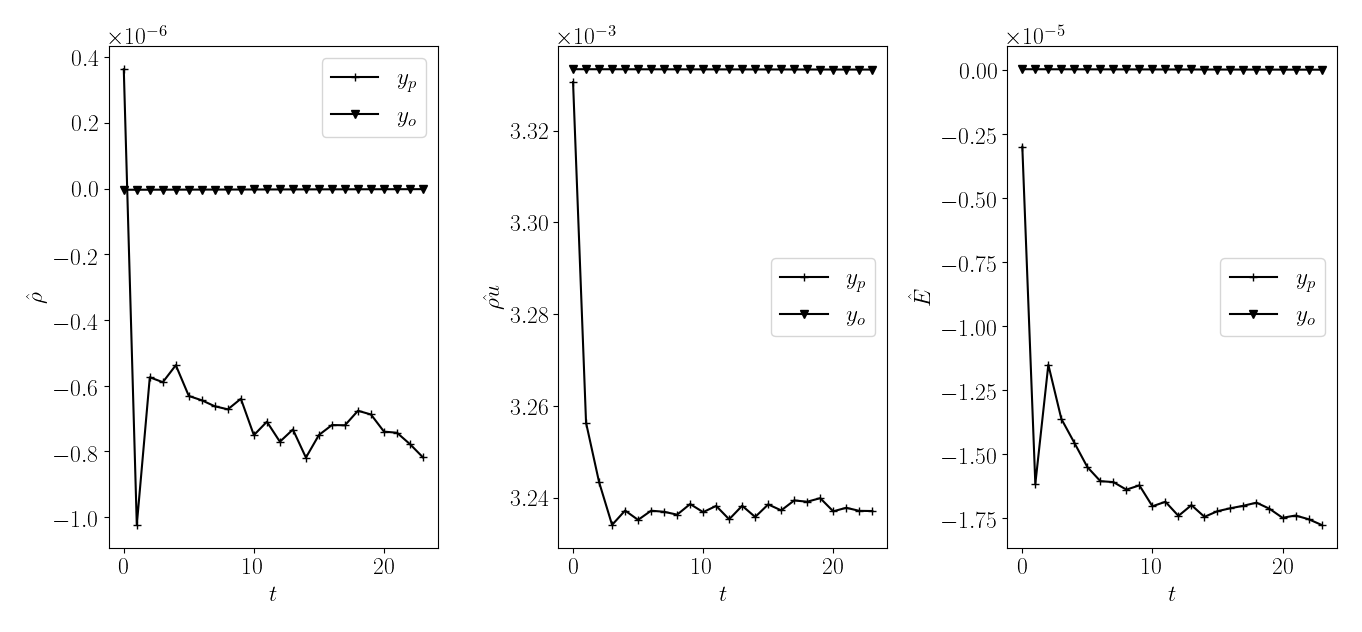
\includegraphics[width=\linewidth]{Figures/02_12_20/kn0p00001Conservative_Quantities/together/all_together.png}
	\caption{Normalized conservative quantities $\hat{\rho}$, $\hat{\rho u}$ and $\hat{E}$ as in \cref{Eq:Norm_Con_quantity} for $y_o$ and $y_p$.}
\end{figure}
\begin{multicols}{2}	
	\begin{equation}
	\hat{\sigma} = \frac{\frac{d}{dt} \int \sigma \,dx}{\bar{\sigma}} = 0 \quad\textrm{and}\quad \bar{\sigma} = \frac{\iint \sigma \,dtdx}{\Delta t}\label{Eq:Norm_Con_quantity}\\
	\end{equation}\break
	\begin{equation}
		L_2 = \frac{||y_o - y_p||}{|||y_o|} \label{L2-Norm}
	\end{equation}
\end{multicols}
Given, that the autoencoder is able to achieve a reconstruction that is equal or below the threshold of the $L_2$-Norm form existing methods like SVD \cref{Sec:SVD} and that conservation is preserved, a reduced order model can not be derived as described in \cref{Sec:Reduced Order Model}. Solely the the reconstuction can be validated. In addition the code needs to be a conservative system hence fulfilling \cref{moment1} to \cref{moment3}.
\begin{figure}
	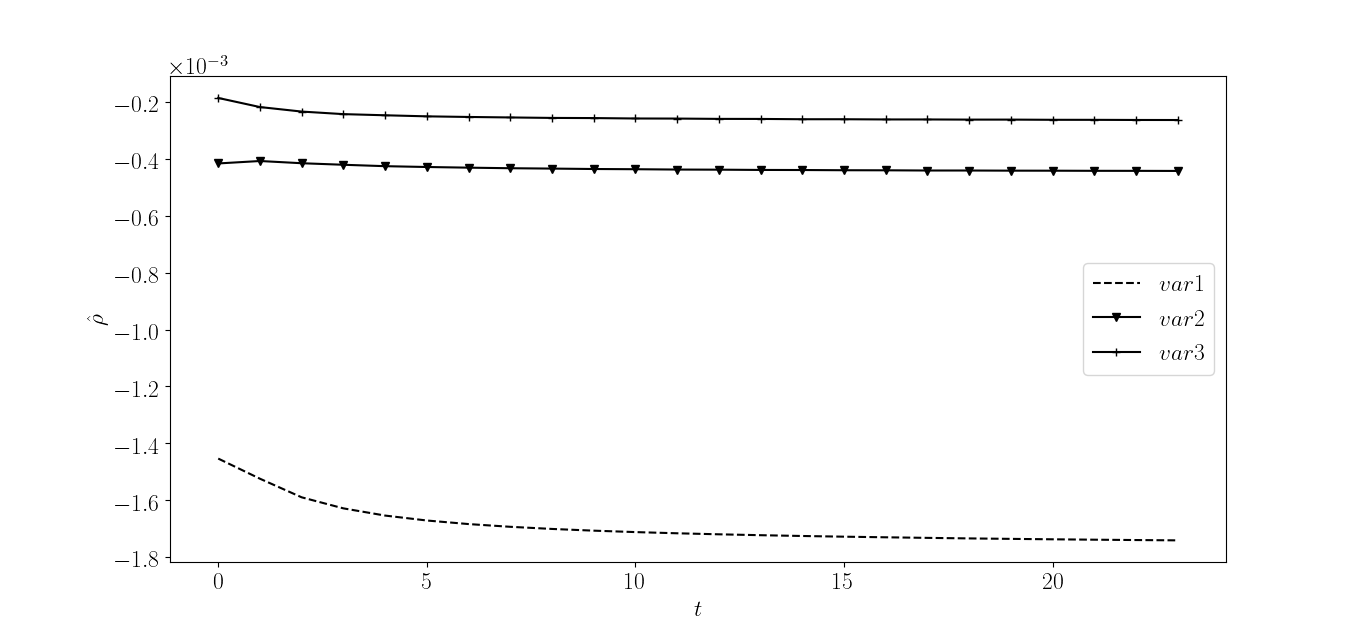
\includegraphics[width=\linewidth]{Figures/02_12_20/kn0p00001Conservative_Quantities/code/Consrvative_Rho_Code.png}
\end{figure}
\begin{figure}[!htbp]
	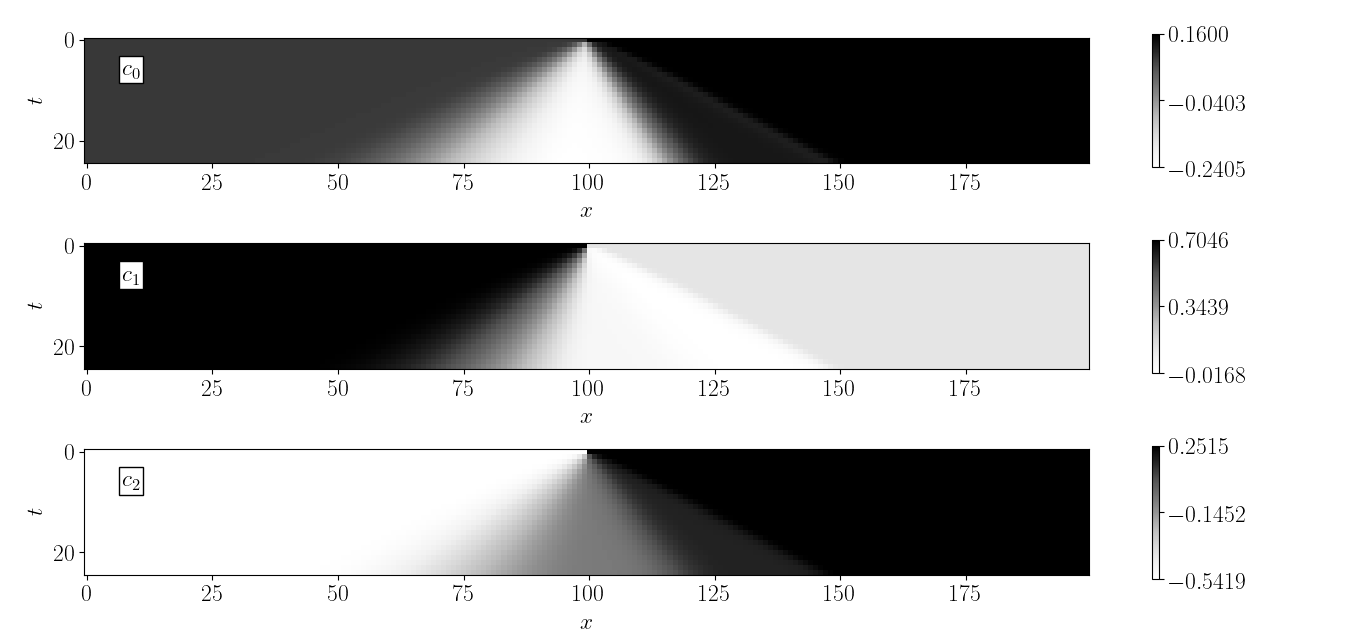
\includegraphics[width=\linewidth]{Figures/Code.png}
	\caption{Code variable $c_1$,$c_2$ and $c_3$ over space $x$ and time $t$ of the fully connected autoencoder}
	\label{Fig:Code_Fully}
\end{figure}
\begin{figure}
	% This file was created by tikzplotlib v0.9.6.
\begin{tikzpicture}

\begin{groupplot}[group style={group size=1 by 3, horizontal sep=2cm, vertical sep=2cm}]
\nextgroupplot[
colorbar,
colorbar style={ylabel={}},
colormap/blackwhite,
point meta max=1,
point meta min=0.124997359296523,
tick align=outside,
tick pos=left,
title={$\rho$},
x grid style={white!69.0196078431373!black},
xlabel={x},
xmin=-0.5, xmax=199.5,
xtick style={color=black},
y grid style={white!69.0196078431373!black},
ylabel={t},
ymin=-0.5, ymax=24.5,
ytick style={color=black},
width=\textwidth,
height=.25\textwidth
]
\addplot graphics [includegraphics cmd=\pgfimage,xmin=-0.5, xmax=199.5, ymin=-0.5, ymax=24.5] {Figures/Results/Macrooriginal-000.png};

\nextgroupplot[
colorbar,
colorbar style={ylabel={}},
colormap/blackwhite,
point meta max=0.975,
point meta min=0.0304687657822372,
tick align=outside,
tick pos=left,
title={E},
x grid style={white!69.0196078431373!black},
xlabel={x},
xmin=-0.5, xmax=199.5,
xtick style={color=black},
y grid style={white!69.0196078431373!black},
ylabel={t},
ymin=-0.5, ymax=24.5,
ytick style={color=black},
width=\textwidth,
height=.25\textwidth
]
\addplot graphics [includegraphics cmd=\pgfimage,xmin=-0.5, xmax=199.5, ymin=-0.5, ymax=24.5] {Figures/Results/Macrooriginal-001.png};

\nextgroupplot[
colorbar,
colorbar style={ylabel={}},
colormap/blackwhite,
point meta max=0.415611533714758,
point meta min=-2.90480106228896e-17,
tick align=outside,
tick pos=left,
title={$\rho$u},
x grid style={white!69.0196078431373!black},
xlabel={x},
xmin=-0.5, xmax=199.5,
xtick style={color=black},
y grid style={white!69.0196078431373!black},
ylabel={t},
ymin=-0.5, ymax=24.5,
ytick style={color=black},
width=\textwidth,
height=.25\textwidth
]
\addplot graphics [includegraphics cmd=\pgfimage,xmin=-0.5, xmax=199.5, ymin=-0.5, ymax=24.5] {Figures/Results/Macrooriginal-002.png};
\end{groupplot}

\end{tikzpicture}

	\caption{Macroscopic quantities $\rho$, E and $\rho$ u of the original data.}
\end{figure}
\begin{figure}[!htbp]
	% This file was created by tikzplotlib v0.9.6.
\begin{tikzpicture}

\begin{groupplot}[group style={group size=3 by 1, horizontal sep=2cm, vertical sep=2cm}]
\nextgroupplot[
tick align=outside,
tick pos=left,
x grid style={white!69.0196078431373!black},
xlabel={t},
xmin=-1.2, xmax=25.2,
xtick style={color=black},
y grid style={white!69.0196078431373!black},
ylabel={u0},
ymin=1611.96396507166, ymax=1966.37809243794,
ytick style={color=black},
width=.3\textwidth,
height=.4\textwidth
]
\addplot [semithick, black, mark=asterisk, mark size=3, mark options={solid}]
table {%
0 1628.07369813376
1 1667.71554096531
2 1743.98141797755
3 1802.36425351953
4 1838.30822493671
5 1862.21684026639
6 1878.96158900469
7 1891.36400083709
8 1900.96567861062
9 1908.56716660305
10 1914.77171625286
11 1919.95306705393
12 1924.3277347325
13 1928.10291753782
14 1931.42597796034
15 1934.34704210956
16 1936.92339749995
17 1939.277117136
18 1941.49313059285
19 1943.47640863995
20 1945.22891375994
21 1946.84995604801
22 1948.32295045775
23 1949.64421744529
24 1950.26835937583
};

\nextgroupplot[
tick align=outside,
tick pos=left,
x grid style={white!69.0196078431373!black},
xlabel={t},
xmin=-1.2, xmax=25.2,
xtick style={color=black},
y grid style={white!69.0196078431373!black},
ylabel={u1},
ymin=-274.389309132333, ymax=-253.272398820019,
ytick style={color=black},
width=.3\textwidth,
height=.4\textwidth
]
\addplot [semithick, black, mark=asterisk, mark size=3, mark options={solid}]
table {%
0 -257.171692592497
1 -254.515300494911
2 -254.272398820019
3 -258.351612389057
4 -261.554906914197
5 -263.985260787298
6 -265.594796024212
7 -266.927943185037
8 -267.937156366821
9 -268.78866243541
10 -269.475127597593
11 -270.06335206048
12 -270.548578231464
13 -270.965438493852
14 -271.345643969425
15 -271.665621043199
16 -271.970152853862
17 -272.271974610773
18 -272.505655020541
19 -272.664732264148
20 -272.862874860928
21 -273.036219893531
22 -273.200434711802
23 -273.33315341083
24 -273.431361022223
};

\nextgroupplot[
tick align=outside,
tick pos=left,
x grid style={white!69.0196078431373!black},
xlabel={t},
xmin=-1.2, xmax=25.2,
xtick style={color=black},
y grid style={white!69.0196078431373!black},
ylabel={u2},
ymin=-45.5377536567457, ymax=-30.6623178468017,
ytick style={color=black},
width=.3\textwidth,
height=.4\textwidth
]
\addplot [semithick, black, mark=asterisk, mark size=3, mark options={solid}]
table {%
0 -31.6623178468017
1 -34.3868975136464
2 -38.4638436013163
3 -40.5821733500112
4 -41.6933777077317
5 -42.3578147737184
6 -42.862631832261
7 -43.1940906634818
8 -43.480635907868
9 -43.6672055719659
10 -43.8381580853925
11 -43.9881808121614
12 -44.1065857660735
13 -44.2134327541779
14 -44.3186696834934
15 -44.4117857444969
16 -44.4744224797722
17 -44.5396918879576
18 -44.5871380898455
19 -44.6321316633901
20 -44.6908604463504
21 -44.7588296817474
22 -44.8091704689491
23 -44.8629326044558
24 -44.8770186181769
};
\end{groupplot}

\end{tikzpicture}

	\caption{Characteristic velocities u0, u1, u2 of the code variables var0, var1, var2 respectively calculated as described in \Cref{Reduced Order Model}.}
\end{figure}
\begin{figure}[!htbp]
	% This file was created by tikzplotlib v0.9.6.
\begin{tikzpicture}

\begin{groupplot}[group style={group size=1 by 3, horizontal sep=2cm, vertical sep=2cm}]
\nextgroupplot[
tick align=outside,
tick pos=left,
title={t=0},
x grid style={white!69.0196078431373!black},
xlabel={x},
xmin=-9.95, xmax=208.95,
xtick style={color=black},
y grid style={white!69.0196078431373!black},
ymin=-0.618888636708649, ymax=1.07585448611601,
ytick style={color=black},
width=\textwidth,
height=.45\textwidth
]
\addplot [semithick, black, dashed]
table {%
0 0.0864763781428337
1 0.0864763781428337
2 0.0864763781428337
3 0.0864763781428337
4 0.0864763781428337
5 0.0864763781428337
6 0.0864763781428337
7 0.0864763781428337
8 0.0864763781428337
9 0.0864763781428337
10 0.0864763781428337
11 0.0864763781428337
12 0.0864763781428337
13 0.0864763781428337
14 0.0864763781428337
15 0.0864763781428337
16 0.0864763781428337
17 0.0864763781428337
18 0.0864763781428337
19 0.0864763781428337
20 0.0864763781428337
21 0.0864763781428337
22 0.0864763781428337
23 0.0864763781428337
24 0.0864763781428337
25 0.0864763781428337
26 0.0864763781428337
27 0.0864763781428337
28 0.0864763781428337
29 0.0864763781428337
30 0.0864763781428337
31 0.0864763781428337
32 0.0864763781428337
33 0.0864763781428337
34 0.0864763781428337
35 0.0864763781428337
36 0.0864763781428337
37 0.0864763781428337
38 0.0864763781428337
39 0.0864763781428337
40 0.0864763781428337
41 0.0864763781428337
42 0.0864763781428337
43 0.0864763781428337
44 0.0864763781428337
45 0.0864763781428337
46 0.0864763781428337
47 0.0864763781428337
48 0.0864763781428337
49 0.0864763781428337
50 0.0864763781428337
51 0.0864763781428337
52 0.0864763781428337
53 0.0864763781428337
54 0.0864763781428337
55 0.0864763781428337
56 0.0864763781428337
57 0.0864763781428337
58 0.0864763781428337
59 0.0864763781428337
60 0.0864763781428337
61 0.0864763781428337
62 0.0864763781428337
63 0.0864763781428337
64 0.0864763781428337
65 0.0864763781428337
66 0.0864763781428337
67 0.0864763781428337
68 0.0864763781428337
69 0.0864763781428337
70 0.0864763781428337
71 0.0864763781428337
72 0.0864763781428337
73 0.0864763781428337
74 0.0864763781428337
75 0.0864763781428337
76 0.0864763781428337
77 0.0864763781428337
78 0.0864763781428337
79 0.0864763781428337
80 0.0864763781428337
81 0.0864763781428337
82 0.0864763781428337
83 0.0864763781428337
84 0.0864763781428337
85 0.0864763781428337
86 0.0864763781428337
87 0.0864763781428337
88 0.0864763781428337
89 0.0864763781428337
90 0.0864763781428337
91 0.0864763781428337
92 0.0864763781428337
93 0.0864763781428337
94 0.0864763781428337
95 0.0864763781428337
96 0.0864763781428337
97 0.0864763781428337
98 0.0864763781428337
99 0.0864763781428337
100 0.159967854619026
101 0.159967854619026
102 0.159967854619026
103 0.159967854619026
104 0.159967854619026
105 0.159967854619026
106 0.159967854619026
107 0.159967854619026
108 0.159967854619026
109 0.159967854619026
110 0.159967854619026
111 0.159967854619026
112 0.159967854619026
113 0.159967854619026
114 0.159967854619026
115 0.159967854619026
116 0.159967854619026
117 0.159967854619026
118 0.159967854619026
119 0.159967854619026
120 0.159967854619026
121 0.159967854619026
122 0.159967854619026
123 0.159967854619026
124 0.159967854619026
125 0.159967854619026
126 0.159967854619026
127 0.159967854619026
128 0.159967854619026
129 0.159967854619026
130 0.159967854619026
131 0.159967854619026
132 0.159967854619026
133 0.159967854619026
134 0.159967854619026
135 0.159967854619026
136 0.159967854619026
137 0.159967854619026
138 0.159967854619026
139 0.159967854619026
140 0.159967854619026
141 0.159967854619026
142 0.159967854619026
143 0.159967854619026
144 0.159967854619026
145 0.159967854619026
146 0.159967854619026
147 0.159967854619026
148 0.159967854619026
149 0.159967854619026
150 0.159967854619026
151 0.159967854619026
152 0.159967854619026
153 0.159967854619026
154 0.159967854619026
155 0.159967854619026
156 0.159967854619026
157 0.159967854619026
158 0.159967854619026
159 0.159967854619026
160 0.159967854619026
161 0.159967854619026
162 0.159967854619026
163 0.159967854619026
164 0.159967854619026
165 0.159967854619026
166 0.159967854619026
167 0.159967854619026
168 0.159967854619026
169 0.159967854619026
170 0.159967854619026
171 0.159967854619026
172 0.159967854619026
173 0.159967854619026
174 0.159967854619026
175 0.159967854619026
176 0.159967854619026
177 0.159967854619026
178 0.159967854619026
179 0.159967854619026
180 0.159967854619026
181 0.159967854619026
182 0.159967854619026
183 0.159967854619026
184 0.159967854619026
185 0.159967854619026
186 0.159967854619026
187 0.159967854619026
188 0.159967854619026
189 0.159967854619026
190 0.159967854619026
191 0.159967854619026
192 0.159967854619026
193 0.159967854619026
194 0.159967854619026
195 0.159967854619026
196 0.159967854619026
197 0.159967854619026
198 0.159967854619026
199 0.159967854619026
};
\addplot [semithick, black]
table {%
0 0.998820707805798
1 0.998820707805798
2 0.998820707805798
3 0.998820707805798
4 0.998820707805798
5 0.998820707805798
6 0.998820707805798
7 0.998820707805798
8 0.998820707805798
9 0.998820707805798
10 0.998820707805798
11 0.998820707805798
12 0.998820707805798
13 0.998820707805798
14 0.998820707805798
15 0.998820707805798
16 0.998820707805798
17 0.998820707805798
18 0.998820707805798
19 0.998820707805798
20 0.998820707805798
21 0.998820707805798
22 0.998820707805798
23 0.998820707805798
24 0.998820707805798
25 0.998820707805798
26 0.998820707805798
27 0.998820707805798
28 0.998820707805798
29 0.998820707805798
30 0.998820707805798
31 0.998820707805798
32 0.998820707805798
33 0.998820707805798
34 0.998820707805798
35 0.998820707805798
36 0.998820707805798
37 0.998820707805798
38 0.998820707805798
39 0.998820707805798
40 0.998820707805798
41 0.998820707805798
42 0.998820707805798
43 0.998820707805798
44 0.998820707805798
45 0.998820707805798
46 0.998820707805798
47 0.998820707805798
48 0.998820707805798
49 0.998820707805798
50 0.998820707805798
51 0.998820707805798
52 0.998820707805798
53 0.998820707805798
54 0.998820707805798
55 0.998820707805798
56 0.998820707805798
57 0.998820707805798
58 0.998820707805798
59 0.998820707805798
60 0.998820707805798
61 0.998820707805798
62 0.998820707805798
63 0.998820707805798
64 0.998820707805798
65 0.998820707805798
66 0.998820707805798
67 0.998820707805798
68 0.998820707805798
69 0.998820707805798
70 0.998820707805798
71 0.998820707805798
72 0.998820707805798
73 0.998820707805798
74 0.998820707805798
75 0.998820707805798
76 0.998820707805798
77 0.998820707805798
78 0.998820707805798
79 0.998820707805798
80 0.998820707805798
81 0.998820707805798
82 0.998820707805798
83 0.998820707805798
84 0.998820707805798
85 0.998820707805798
86 0.998820707805798
87 0.998820707805798
88 0.998820707805798
89 0.998820707805798
90 0.998820707805798
91 0.998820707805798
92 0.998820707805798
93 0.998820707805798
94 0.998820707805798
95 0.998820707805798
96 0.998820707805798
97 0.998820707805798
98 0.998820707805798
99 0.998820707805798
100 0.124468828688082
101 0.124468828688082
102 0.124468828688082
103 0.124468828688082
104 0.124468828688082
105 0.124468828688082
106 0.124468828688082
107 0.124468828688082
108 0.124468828688082
109 0.124468828688082
110 0.124468828688082
111 0.124468828688082
112 0.124468828688082
113 0.124468828688082
114 0.124468828688082
115 0.124468828688082
116 0.124468828688082
117 0.124468828688082
118 0.124468828688082
119 0.124468828688082
120 0.124468828688082
121 0.124468828688082
122 0.124468828688082
123 0.124468828688082
124 0.124468828688082
125 0.124468828688082
126 0.124468828688082
127 0.124468828688082
128 0.124468828688082
129 0.124468828688082
130 0.124468828688082
131 0.124468828688082
132 0.124468828688082
133 0.124468828688082
134 0.124468828688082
135 0.124468828688082
136 0.124468828688082
137 0.124468828688082
138 0.124468828688082
139 0.124468828688082
140 0.124468828688082
141 0.124468828688082
142 0.124468828688082
143 0.124468828688082
144 0.124468828688082
145 0.124468828688082
146 0.124468828688082
147 0.124468828688082
148 0.124468828688082
149 0.124468828688082
150 0.124468828688082
151 0.124468828688082
152 0.124468828688082
153 0.124468828688082
154 0.124468828688082
155 0.124468828688082
156 0.124468828688082
157 0.124468828688082
158 0.124468828688082
159 0.124468828688082
160 0.124468828688082
161 0.124468828688082
162 0.124468828688082
163 0.124468828688082
164 0.124468828688082
165 0.124468828688082
166 0.124468828688082
167 0.124468828688082
168 0.124468828688082
169 0.124468828688082
170 0.124468828688082
171 0.124468828688082
172 0.124468828688082
173 0.124468828688082
174 0.124468828688082
175 0.124468828688082
176 0.124468828688082
177 0.124468828688082
178 0.124468828688082
179 0.124468828688082
180 0.124468828688082
181 0.124468828688082
182 0.124468828688082
183 0.124468828688082
184 0.124468828688082
185 0.124468828688082
186 0.124468828688082
187 0.124468828688082
188 0.124468828688082
189 0.124468828688082
190 0.124468828688082
191 0.124468828688082
192 0.124468828688082
193 0.124468828688082
194 0.124468828688082
195 0.124468828688082
196 0.124468828688082
197 0.124468828688082
198 0.124468828688082
199 0.124468828688082
};
\addplot [semithick, black, dashed]
table {%
0 0.704569160938263
1 0.704569160938263
2 0.704569160938263
3 0.704569160938263
4 0.704569160938263
5 0.704569160938263
6 0.704569160938263
7 0.704569160938263
8 0.704569160938263
9 0.704569160938263
10 0.704569160938263
11 0.704569160938263
12 0.704569160938263
13 0.704569160938263
14 0.704569160938263
15 0.704569160938263
16 0.704569160938263
17 0.704569160938263
18 0.704569160938263
19 0.704569160938263
20 0.704569160938263
21 0.704569160938263
22 0.704569160938263
23 0.704569160938263
24 0.704569160938263
25 0.704569160938263
26 0.704569160938263
27 0.704569160938263
28 0.704569160938263
29 0.704569160938263
30 0.704569160938263
31 0.704569160938263
32 0.704569160938263
33 0.704569160938263
34 0.704569160938263
35 0.704569160938263
36 0.704569160938263
37 0.704569160938263
38 0.704569160938263
39 0.704569160938263
40 0.704569160938263
41 0.704569160938263
42 0.704569160938263
43 0.704569160938263
44 0.704569160938263
45 0.704569160938263
46 0.704569160938263
47 0.704569160938263
48 0.704569160938263
49 0.704569160938263
50 0.704569160938263
51 0.704569160938263
52 0.704569160938263
53 0.704569160938263
54 0.704569160938263
55 0.704569160938263
56 0.704569160938263
57 0.704569160938263
58 0.704569160938263
59 0.704569160938263
60 0.704569160938263
61 0.704569160938263
62 0.704569160938263
63 0.704569160938263
64 0.704569160938263
65 0.704569160938263
66 0.704569160938263
67 0.704569160938263
68 0.704569160938263
69 0.704569160938263
70 0.704569160938263
71 0.704569160938263
72 0.704569160938263
73 0.704569160938263
74 0.704569160938263
75 0.704569160938263
76 0.704569160938263
77 0.704569160938263
78 0.704569160938263
79 0.704569160938263
80 0.704569160938263
81 0.704569160938263
82 0.704569160938263
83 0.704569160938263
84 0.704569160938263
85 0.704569160938263
86 0.704569160938263
87 0.704569160938263
88 0.704569160938263
89 0.704569160938263
90 0.704569160938263
91 0.704569160938263
92 0.704569160938263
93 0.704569160938263
94 0.704569160938263
95 0.704569160938263
96 0.704569160938263
97 0.704569160938263
98 0.704569160938263
99 0.704569160938263
100 0.116299636662006
101 0.116299636662006
102 0.116299636662006
103 0.116299636662006
104 0.116299636662006
105 0.116299636662006
106 0.116299636662006
107 0.116299636662006
108 0.116299636662006
109 0.116299636662006
110 0.116299636662006
111 0.116299636662006
112 0.116299636662006
113 0.116299636662006
114 0.116299636662006
115 0.116299636662006
116 0.116299636662006
117 0.116299636662006
118 0.116299636662006
119 0.116299636662006
120 0.116299636662006
121 0.116299636662006
122 0.116299636662006
123 0.116299636662006
124 0.116299636662006
125 0.116299636662006
126 0.116299636662006
127 0.116299636662006
128 0.116299636662006
129 0.116299636662006
130 0.116299636662006
131 0.116299636662006
132 0.116299636662006
133 0.116299636662006
134 0.116299636662006
135 0.116299636662006
136 0.116299636662006
137 0.116299636662006
138 0.116299636662006
139 0.116299636662006
140 0.116299636662006
141 0.116299636662006
142 0.116299636662006
143 0.116299636662006
144 0.116299636662006
145 0.116299636662006
146 0.116299636662006
147 0.116299636662006
148 0.116299636662006
149 0.116299636662006
150 0.116299636662006
151 0.116299636662006
152 0.116299636662006
153 0.116299636662006
154 0.116299636662006
155 0.116299636662006
156 0.116299636662006
157 0.116299636662006
158 0.116299636662006
159 0.116299636662006
160 0.116299636662006
161 0.116299636662006
162 0.116299636662006
163 0.116299636662006
164 0.116299636662006
165 0.116299636662006
166 0.116299636662006
167 0.116299636662006
168 0.116299636662006
169 0.116299636662006
170 0.116299636662006
171 0.116299636662006
172 0.116299636662006
173 0.116299636662006
174 0.116299636662006
175 0.116299636662006
176 0.116299636662006
177 0.116299636662006
178 0.116299636662006
179 0.116299636662006
180 0.116299636662006
181 0.116299636662006
182 0.116299636662006
183 0.116299636662006
184 0.116299636662006
185 0.116299636662006
186 0.116299636662006
187 0.116299636662006
188 0.116299636662006
189 0.116299636662006
190 0.116299636662006
191 0.116299636662006
192 0.116299636662006
193 0.116299636662006
194 0.116299636662006
195 0.116299636662006
196 0.116299636662006
197 0.116299636662006
198 0.116299636662006
199 0.116299636662006
};
\addplot [semithick, black]
table {%
0 0.957552853847665
1 0.957552853847665
2 0.957552853847665
3 0.957552853847665
4 0.957552853847665
5 0.957552853847665
6 0.957552853847665
7 0.957552853847665
8 0.957552853847665
9 0.957552853847665
10 0.957552853847665
11 0.957552853847665
12 0.957552853847665
13 0.957552853847665
14 0.957552853847665
15 0.957552853847665
16 0.957552853847665
17 0.957552853847665
18 0.957552853847665
19 0.957552853847665
20 0.957552853847665
21 0.957552853847665
22 0.957552853847665
23 0.957552853847665
24 0.957552853847665
25 0.957552853847665
26 0.957552853847665
27 0.957552853847665
28 0.957552853847665
29 0.957552853847665
30 0.957552853847665
31 0.957552853847665
32 0.957552853847665
33 0.957552853847665
34 0.957552853847665
35 0.957552853847665
36 0.957552853847665
37 0.957552853847665
38 0.957552853847665
39 0.957552853847665
40 0.957552853847665
41 0.957552853847665
42 0.957552853847665
43 0.957552853847665
44 0.957552853847665
45 0.957552853847665
46 0.957552853847665
47 0.957552853847665
48 0.957552853847665
49 0.957552853847665
50 0.957552853847665
51 0.957552853847665
52 0.957552853847665
53 0.957552853847665
54 0.957552853847665
55 0.957552853847665
56 0.957552853847665
57 0.957552853847665
58 0.957552853847665
59 0.957552853847665
60 0.957552853847665
61 0.957552853847665
62 0.957552853847665
63 0.957552853847665
64 0.957552853847665
65 0.957552853847665
66 0.957552853847665
67 0.957552853847665
68 0.957552853847665
69 0.957552853847665
70 0.957552853847665
71 0.957552853847665
72 0.957552853847665
73 0.957552853847665
74 0.957552853847665
75 0.957552853847665
76 0.957552853847665
77 0.957552853847665
78 0.957552853847665
79 0.957552853847665
80 0.957552853847665
81 0.957552853847665
82 0.957552853847665
83 0.957552853847665
84 0.957552853847665
85 0.957552853847665
86 0.957552853847665
87 0.957552853847665
88 0.957552853847665
89 0.957552853847665
90 0.957552853847665
91 0.957552853847665
92 0.957552853847665
93 0.957552853847665
94 0.957552853847665
95 0.957552853847665
96 0.957552853847665
97 0.957552853847665
98 0.957552853847665
99 0.957552853847665
100 0.0208907090440876
101 0.0208907090440876
102 0.0208907090440876
103 0.0208907090440876
104 0.0208907090440876
105 0.0208907090440876
106 0.0208907090440876
107 0.0208907090440876
108 0.0208907090440876
109 0.0208907090440876
110 0.0208907090440876
111 0.0208907090440876
112 0.0208907090440876
113 0.0208907090440876
114 0.0208907090440876
115 0.0208907090440876
116 0.0208907090440876
117 0.0208907090440876
118 0.0208907090440876
119 0.0208907090440876
120 0.0208907090440876
121 0.0208907090440876
122 0.0208907090440876
123 0.0208907090440876
124 0.0208907090440876
125 0.0208907090440876
126 0.0208907090440876
127 0.0208907090440876
128 0.0208907090440876
129 0.0208907090440876
130 0.0208907090440876
131 0.0208907090440876
132 0.0208907090440876
133 0.0208907090440876
134 0.0208907090440876
135 0.0208907090440876
136 0.0208907090440876
137 0.0208907090440876
138 0.0208907090440876
139 0.0208907090440876
140 0.0208907090440876
141 0.0208907090440876
142 0.0208907090440876
143 0.0208907090440876
144 0.0208907090440876
145 0.0208907090440876
146 0.0208907090440876
147 0.0208907090440876
148 0.0208907090440876
149 0.0208907090440876
150 0.0208907090440876
151 0.0208907090440876
152 0.0208907090440876
153 0.0208907090440876
154 0.0208907090440876
155 0.0208907090440876
156 0.0208907090440876
157 0.0208907090440876
158 0.0208907090440876
159 0.0208907090440876
160 0.0208907090440876
161 0.0208907090440876
162 0.0208907090440876
163 0.0208907090440876
164 0.0208907090440876
165 0.0208907090440876
166 0.0208907090440876
167 0.0208907090440876
168 0.0208907090440876
169 0.0208907090440876
170 0.0208907090440876
171 0.0208907090440876
172 0.0208907090440876
173 0.0208907090440876
174 0.0208907090440876
175 0.0208907090440876
176 0.0208907090440876
177 0.0208907090440876
178 0.0208907090440876
179 0.0208907090440876
180 0.0208907090440876
181 0.0208907090440876
182 0.0208907090440876
183 0.0208907090440876
184 0.0208907090440876
185 0.0208907090440876
186 0.0208907090440876
187 0.0208907090440876
188 0.0208907090440876
189 0.0208907090440876
190 0.0208907090440876
191 0.0208907090440876
192 0.0208907090440876
193 0.0208907090440876
194 0.0208907090440876
195 0.0208907090440876
196 0.0208907090440876
197 0.0208907090440876
198 0.0208907090440876
199 0.0208907090440876
};
\addplot [semithick, black, dashed]
table {%
0 -0.541854858398438
1 -0.541854858398438
2 -0.541854858398438
3 -0.541854858398438
4 -0.541854858398438
5 -0.541854858398438
6 -0.541854858398438
7 -0.541854858398438
8 -0.541854858398438
9 -0.541854858398438
10 -0.541854858398438
11 -0.541854858398438
12 -0.541854858398438
13 -0.541854858398438
14 -0.541854858398438
15 -0.541854858398438
16 -0.541854858398438
17 -0.541854858398438
18 -0.541854858398438
19 -0.541854858398438
20 -0.541854858398438
21 -0.541854858398438
22 -0.541854858398438
23 -0.541854858398438
24 -0.541854858398438
25 -0.541854858398438
26 -0.541854858398438
27 -0.541854858398438
28 -0.541854858398438
29 -0.541854858398438
30 -0.541854858398438
31 -0.541854858398438
32 -0.541854858398438
33 -0.541854858398438
34 -0.541854858398438
35 -0.541854858398438
36 -0.541854858398438
37 -0.541854858398438
38 -0.541854858398438
39 -0.541854858398438
40 -0.541854858398438
41 -0.541854858398438
42 -0.541854858398438
43 -0.541854858398438
44 -0.541854858398438
45 -0.541854858398438
46 -0.541854858398438
47 -0.541854858398438
48 -0.541854858398438
49 -0.541854858398438
50 -0.541854858398438
51 -0.541854858398438
52 -0.541854858398438
53 -0.541854858398438
54 -0.541854858398438
55 -0.541854858398438
56 -0.541854858398438
57 -0.541854858398438
58 -0.541854858398438
59 -0.541854858398438
60 -0.541854858398438
61 -0.541854858398438
62 -0.541854858398438
63 -0.541854858398438
64 -0.541854858398438
65 -0.541854858398438
66 -0.541854858398438
67 -0.541854858398438
68 -0.541854858398438
69 -0.541854858398438
70 -0.541854858398438
71 -0.541854858398438
72 -0.541854858398438
73 -0.541854858398438
74 -0.541854858398438
75 -0.541854858398438
76 -0.541854858398438
77 -0.541854858398438
78 -0.541854858398438
79 -0.541854858398438
80 -0.541854858398438
81 -0.541854858398438
82 -0.541854858398438
83 -0.541854858398438
84 -0.541854858398438
85 -0.541854858398438
86 -0.541854858398438
87 -0.541854858398438
88 -0.541854858398438
89 -0.541854858398438
90 -0.541854858398438
91 -0.541854858398438
92 -0.541854858398438
93 -0.541854858398438
94 -0.541854858398438
95 -0.541854858398438
96 -0.541854858398438
97 -0.541854858398438
98 -0.541854858398438
99 -0.541854858398438
100 0.251547485589981
101 0.251547485589981
102 0.251547485589981
103 0.251547485589981
104 0.251547485589981
105 0.251547485589981
106 0.251547485589981
107 0.251547485589981
108 0.251547485589981
109 0.251547485589981
110 0.251547485589981
111 0.251547485589981
112 0.251547485589981
113 0.251547485589981
114 0.251547485589981
115 0.251547485589981
116 0.251547485589981
117 0.251547485589981
118 0.251547485589981
119 0.251547485589981
120 0.251547485589981
121 0.251547485589981
122 0.251547485589981
123 0.251547485589981
124 0.251547485589981
125 0.251547485589981
126 0.251547485589981
127 0.251547485589981
128 0.251547485589981
129 0.251547485589981
130 0.251547485589981
131 0.251547485589981
132 0.251547485589981
133 0.251547485589981
134 0.251547485589981
135 0.251547485589981
136 0.251547485589981
137 0.251547485589981
138 0.251547485589981
139 0.251547485589981
140 0.251547485589981
141 0.251547485589981
142 0.251547485589981
143 0.251547485589981
144 0.251547485589981
145 0.251547485589981
146 0.251547485589981
147 0.251547485589981
148 0.251547485589981
149 0.251547485589981
150 0.251547485589981
151 0.251547485589981
152 0.251547485589981
153 0.251547485589981
154 0.251547485589981
155 0.251547485589981
156 0.251547485589981
157 0.251547485589981
158 0.251547485589981
159 0.251547485589981
160 0.251547485589981
161 0.251547485589981
162 0.251547485589981
163 0.251547485589981
164 0.251547485589981
165 0.251547485589981
166 0.251547485589981
167 0.251547485589981
168 0.251547485589981
169 0.251547485589981
170 0.251547485589981
171 0.251547485589981
172 0.251547485589981
173 0.251547485589981
174 0.251547485589981
175 0.251547485589981
176 0.251547485589981
177 0.251547485589981
178 0.251547485589981
179 0.251547485589981
180 0.251547485589981
181 0.251547485589981
182 0.251547485589981
183 0.251547485589981
184 0.251547485589981
185 0.251547485589981
186 0.251547485589981
187 0.251547485589981
188 0.251547485589981
189 0.251547485589981
190 0.251547485589981
191 0.251547485589981
192 0.251547485589981
193 0.251547485589981
194 0.251547485589981
195 0.251547485589981
196 0.251547485589981
197 0.251547485589981
198 0.251547485589981
199 0.251547485589981
};
\addplot [semithick, black]
table {%
0 0.00276484748660005
1 0.00276484748660005
2 0.00276484748660005
3 0.00276484748660005
4 0.00276484748660005
5 0.00276484748660005
6 0.00276484748660005
7 0.00276484748660005
8 0.00276484748660005
9 0.00276484748660005
10 0.00276484748660005
11 0.00276484748660005
12 0.00276484748660005
13 0.00276484748660005
14 0.00276484748660005
15 0.00276484748660005
16 0.00276484748660005
17 0.00276484748660005
18 0.00276484748660005
19 0.00276484748660005
20 0.00276484748660005
21 0.00276484748660005
22 0.00276484748660005
23 0.00276484748660005
24 0.00276484748660005
25 0.00276484748660005
26 0.00276484748660005
27 0.00276484748660005
28 0.00276484748660005
29 0.00276484748660005
30 0.00276484748660005
31 0.00276484748660005
32 0.00276484748660005
33 0.00276484748660005
34 0.00276484748660005
35 0.00276484748660005
36 0.00276484748660005
37 0.00276484748660005
38 0.00276484748660005
39 0.00276484748660005
40 0.00276484748660005
41 0.00276484748660005
42 0.00276484748660005
43 0.00276484748660005
44 0.00276484748660005
45 0.00276484748660005
46 0.00276484748660005
47 0.00276484748660005
48 0.00276484748660005
49 0.00276484748660005
50 0.00276484748660005
51 0.00276484748660005
52 0.00276484748660005
53 0.00276484748660005
54 0.00276484748660005
55 0.00276484748660005
56 0.00276484748660005
57 0.00276484748660005
58 0.00276484748660005
59 0.00276484748660005
60 0.00276484748660005
61 0.00276484748660005
62 0.00276484748660005
63 0.00276484748660005
64 0.00276484748660005
65 0.00276484748660005
66 0.00276484748660005
67 0.00276484748660005
68 0.00276484748660005
69 0.00276484748660005
70 0.00276484748660005
71 0.00276484748660005
72 0.00276484748660005
73 0.00276484748660005
74 0.00276484748660005
75 0.00276484748660005
76 0.00276484748660005
77 0.00276484748660005
78 0.00276484748660005
79 0.00276484748660005
80 0.00276484748660005
81 0.00276484748660005
82 0.00276484748660005
83 0.00276484748660005
84 0.00276484748660005
85 0.00276484748660005
86 0.00276484748660005
87 0.00276484748660005
88 0.00276484748660005
89 0.00276484748660005
90 0.00276484748660005
91 0.00276484748660005
92 0.00276484748660005
93 0.00276484748660005
94 0.00276484748660005
95 0.00276484748660005
96 0.00276484748660005
97 0.00276484748660005
98 0.00276484748660005
99 0.00276484748660005
100 0.000327279684018397
101 0.000327279684018397
102 0.000327279684018397
103 0.000327279684018397
104 0.000327279684018397
105 0.000327279684018397
106 0.000327279684018397
107 0.000327279684018397
108 0.000327279684018397
109 0.000327279684018397
110 0.000327279684018397
111 0.000327279684018397
112 0.000327279684018397
113 0.000327279684018397
114 0.000327279684018397
115 0.000327279684018397
116 0.000327279684018397
117 0.000327279684018397
118 0.000327279684018397
119 0.000327279684018397
120 0.000327279684018397
121 0.000327279684018397
122 0.000327279684018397
123 0.000327279684018397
124 0.000327279684018397
125 0.000327279684018397
126 0.000327279684018397
127 0.000327279684018397
128 0.000327279684018397
129 0.000327279684018397
130 0.000327279684018397
131 0.000327279684018397
132 0.000327279684018397
133 0.000327279684018397
134 0.000327279684018397
135 0.000327279684018397
136 0.000327279684018397
137 0.000327279684018397
138 0.000327279684018397
139 0.000327279684018397
140 0.000327279684018397
141 0.000327279684018397
142 0.000327279684018397
143 0.000327279684018397
144 0.000327279684018397
145 0.000327279684018397
146 0.000327279684018397
147 0.000327279684018397
148 0.000327279684018397
149 0.000327279684018397
150 0.000327279684018397
151 0.000327279684018397
152 0.000327279684018397
153 0.000327279684018397
154 0.000327279684018397
155 0.000327279684018397
156 0.000327279684018397
157 0.000327279684018397
158 0.000327279684018397
159 0.000327279684018397
160 0.000327279684018397
161 0.000327279684018397
162 0.000327279684018397
163 0.000327279684018397
164 0.000327279684018397
165 0.000327279684018397
166 0.000327279684018397
167 0.000327279684018397
168 0.000327279684018397
169 0.000327279684018397
170 0.000327279684018397
171 0.000327279684018397
172 0.000327279684018397
173 0.000327279684018397
174 0.000327279684018397
175 0.000327279684018397
176 0.000327279684018397
177 0.000327279684018397
178 0.000327279684018397
179 0.000327279684018397
180 0.000327279684018397
181 0.000327279684018397
182 0.000327279684018397
183 0.000327279684018397
184 0.000327279684018397
185 0.000327279684018397
186 0.000327279684018397
187 0.000327279684018397
188 0.000327279684018397
189 0.000327279684018397
190 0.000327279684018397
191 0.000327279684018397
192 0.000327279684018397
193 0.000327279684018397
194 0.000327279684018397
195 0.000327279684018397
196 0.000327279684018397
197 0.000327279684018397
198 0.000327279684018397
199 0.000327279684018397
};

\nextgroupplot[
tick align=outside,
tick pos=left,
title={t=10},
x grid style={white!69.0196078431373!black},
xlabel={x},
xmin=-9.95, xmax=208.95,
xtick style={color=black},
y grid style={white!69.0196078431373!black},
ymin=-0.618888640008754, ymax=1.0758545554182,
ytick style={color=black},
width=\textwidth,
height=.45\textwidth
]
\addplot [semithick, black, dashed]
table {%
0 0.0864763781428337
1 0.0864763781428337
2 0.0864763781428337
3 0.0864763781428337
4 0.0864763781428337
5 0.0864763781428337
6 0.0864763781428337
7 0.0864763781428337
8 0.0864763781428337
9 0.0864763781428337
10 0.0864763781428337
11 0.0864763781428337
12 0.0864763781428337
13 0.0864763781428337
14 0.0864763781428337
15 0.0864763781428337
16 0.0864763781428337
17 0.0864763781428337
18 0.0864763781428337
19 0.0864763781428337
20 0.0864763781428337
21 0.0864763781428337
22 0.0864763781428337
23 0.0864763781428337
24 0.0864763781428337
25 0.0864763781428337
26 0.0864763781428337
27 0.0864763781428337
28 0.0864763781428337
29 0.0864763781428337
30 0.0864763781428337
31 0.0864763781428337
32 0.0864763781428337
33 0.0864763781428337
34 0.0864763781428337
35 0.0864763781428337
36 0.0864763781428337
37 0.0864763781428337
38 0.0864763781428337
39 0.0864763781428337
40 0.0864763781428337
41 0.0864763781428337
42 0.0864763781428337
43 0.0864763781428337
44 0.0864763781428337
45 0.0864763781428337
46 0.0864763781428337
47 0.0864763781428337
48 0.0864763781428337
49 0.0864763781428337
50 0.0864763781428337
51 0.0864763781428337
52 0.0864763781428337
53 0.0864763781428337
54 0.0864763781428337
55 0.0864763781428337
56 0.0864763706922531
57 0.0864763334393501
58 0.0864762738347054
59 0.0864761620759964
60 0.0864758640527725
61 0.0864753127098083
62 0.0864739865064621
63 0.0864712372422218
64 0.0864655897021294
65 0.0864543095231056
66 0.0864325016736984
67 0.0863915756344795
68 0.0863169431686401
69 0.0861852243542671
70 0.0859597772359848
71 0.0855867117643356
72 0.0849898457527161
73 0.0840671584010124
74 0.0826498940587044
75 0.0803875625133514
76 0.077234223484993
77 0.072984017431736
78 0.0674387067556381
79 0.0604246556758881
80 0.0518089793622494
81 0.0415117479860783
82 0.0295130852609873
83 0.0158548932522535
84 0.0006373300566338
85 -0.015987241640687
86 -0.0338233225047588
87 -0.0526409223675728
88 -0.07218337059021
89 -0.0921719744801521
90 -0.112306721508503
91 -0.132261112332344
92 -0.151669800281525
93 -0.170107528567314
94 -0.187061071395874
95 -0.20189805328846
96 -0.21385258436203
97 -0.222053498029709
98 -0.225772872567177
99 -0.224780276417732
100 -0.219312369823456
101 -0.209041133522987
102 -0.191329523921013
103 -0.163140207529068
104 -0.123704329133034
105 -0.076011136174202
106 -0.0262000784277916
107 0.0194125380367041
108 0.0566670969128609
109 0.0843709632754326
110 0.103447303175926
111 0.115707568824291
112 0.123025268316269
113 0.126965016126633
114 0.128674626350403
115 0.128887668251991
116 0.127975702285767
117 0.126061379909515
118 0.123282037675381
119 0.120394363999367
120 0.119689486920834
121 0.125713557004929
122 0.139865666627884
123 0.152246356010437
124 0.157710343599319
125 0.159378811717033
126 0.1598189920187
127 0.159929275512695
128 0.159956306219101
129 0.159962862730026
130 0.159964442253113
131 0.159964799880981
132 0.159964889287949
133 0.159964919090271
134 0.159964919090271
135 0.159964919090271
136 0.159964919090271
137 0.159964919090271
138 0.159964919090271
139 0.159964919090271
140 0.159964919090271
141 0.159964919090271
142 0.159964919090271
143 0.159964919090271
144 0.159964919090271
145 0.159964919090271
146 0.159964919090271
147 0.159964919090271
148 0.159964919090271
149 0.159964919090271
150 0.159964919090271
151 0.159964919090271
152 0.159964919090271
153 0.159964919090271
154 0.159964919090271
155 0.159964919090271
156 0.159964919090271
157 0.159964919090271
158 0.159964919090271
159 0.159964919090271
160 0.159964919090271
161 0.159964919090271
162 0.159964919090271
163 0.159964919090271
164 0.159964919090271
165 0.159964919090271
166 0.159964919090271
167 0.159964919090271
168 0.159964919090271
169 0.159964919090271
170 0.159964919090271
171 0.159964919090271
172 0.159964919090271
173 0.159964919090271
174 0.159964919090271
175 0.159964919090271
176 0.159964919090271
177 0.159964919090271
178 0.159964919090271
179 0.159964919090271
180 0.159964919090271
181 0.159964919090271
182 0.159964919090271
183 0.159964919090271
184 0.159964919090271
185 0.159964919090271
186 0.159964919090271
187 0.159964919090271
188 0.159964919090271
189 0.159964919090271
190 0.159964919090271
191 0.159964919090271
192 0.159964919090271
193 0.159964919090271
194 0.159964919090271
195 0.159964919090271
196 0.159964919090271
197 0.159964919090271
198 0.159964919090271
199 0.159964919090271
};
\addplot [semithick, black]
table {%
0 0.998820707805798
1 0.998820707805798
2 0.998820707805798
3 0.998820707805798
4 0.998820707805798
5 0.998820707805798
6 0.998820707805798
7 0.998820707805798
8 0.998820707805798
9 0.998820707805798
10 0.998820707805798
11 0.998820707805798
12 0.998820707805798
13 0.998820707805798
14 0.998820707805798
15 0.998820707805798
16 0.998820707805798
17 0.998820707805798
18 0.998820707805798
19 0.998820707805798
20 0.998820707805798
21 0.998820707805798
22 0.998820707805798
23 0.998820707805798
24 0.998820707805798
25 0.998820707805798
26 0.998820707805798
27 0.998820707805798
28 0.998820707805798
29 0.998820707805798
30 0.998820707805798
31 0.998820707805798
32 0.998820707805798
33 0.998820707805798
34 0.998820707805798
35 0.998820707805798
36 0.998820707805798
37 0.998820707805798
38 0.998820707805798
39 0.998820707805798
40 0.998820707805798
41 0.998820707805798
42 0.998820707805798
43 0.998820707805798
44 0.998820707805798
45 0.998820707805798
46 0.998820707805798
47 0.998820707805798
48 0.998820707805798
49 0.998820707805798
50 0.998820707805798
51 0.998820707805798
52 0.998820707805798
53 0.998820707805798
54 0.998820707805798
55 0.998820707805798
56 0.998820760291134
57 0.998820773807887
58 0.998820724033428
59 0.998820498134271
60 0.998820354072147
61 0.998819787491957
62 0.998818709993266
63 0.998816438867519
64 0.998811647653366
65 0.998802133932894
66 0.998783784556689
67 0.998749135413204
68 0.998685901983972
69 0.998573943772108
70 0.998382093047095
71 0.99806367534647
72 0.99755233596683
73 0.996758791228966
74 0.995562235864764
75 0.993795790222888
76 0.991312451792947
77 0.987930607509993
78 0.983461891827346
79 0.977723691639446
80 0.970549134859547
81 0.96179809916837
82 0.951367633436214
83 0.939189634603496
84 0.925419590008629
85 0.910015075847446
86 0.892986014455346
87 0.874414008147095
88 0.854575300913485
89 0.833530392317826
90 0.811196551657047
91 0.787644835338538
92 0.762925393836877
93 0.737093863691496
94 0.710239872576506
95 0.682530534706518
96 0.654519607214052
97 0.627513133201249
98 0.602692004498784
99 0.581505205990745
100 0.564988579789525
101 0.551121995186361
102 0.534104219966768
103 0.508901579789661
104 0.473503964586155
105 0.429484190838663
106 0.380857970886953
107 0.333951645265281
108 0.293033010955941
109 0.260566858589113
110 0.236948914774378
111 0.221048299986834
112 0.211176159217967
113 0.205497573825153
114 0.202345116911322
115 0.200305667236441
116 0.198136378712661
117 0.194655276853458
118 0.188450423047004
119 0.177507850479136
120 0.162286801397642
121 0.14817348059739
122 0.136511400662351
123 0.129026887965
124 0.125828234000402
125 0.124826781878442
126 0.124558060439283
127 0.124490321391897
128 0.124473699448391
129 0.124469624696705
130 0.124468652921643
131 0.124468480856789
132 0.124468422541854
133 0.124468384792402
134 0.124468384792402
135 0.124468384792402
136 0.124468384792402
137 0.124468384792402
138 0.124468384792402
139 0.124468384792402
140 0.124468384792402
141 0.124468384792402
142 0.124468384792402
143 0.124468384792402
144 0.124468384792402
145 0.124468384792402
146 0.124468384792402
147 0.124468384792402
148 0.124468384792402
149 0.124468384792402
150 0.124468384792402
151 0.124468384792402
152 0.124468384792402
153 0.124468384792402
154 0.124468384792402
155 0.124468384792402
156 0.124468384792402
157 0.124468384792402
158 0.124468384792402
159 0.124468384792402
160 0.124468384792402
161 0.124468384792402
162 0.124468384792402
163 0.124468384792402
164 0.124468384792402
165 0.124468384792402
166 0.124468384792402
167 0.124468384792402
168 0.124468384792402
169 0.124468384792402
170 0.124468384792402
171 0.124468384792402
172 0.124468384792402
173 0.124468384792402
174 0.124468384792402
175 0.124468384792402
176 0.124468384792402
177 0.124468384792402
178 0.124468384792402
179 0.124468384792402
180 0.124468384792402
181 0.124468384792402
182 0.124468384792402
183 0.124468384792402
184 0.124468384792402
185 0.124468384792402
186 0.124468384792402
187 0.124468384792402
188 0.124468384792402
189 0.124468384792402
190 0.124468384792402
191 0.124468384792402
192 0.124468384792402
193 0.124468384792402
194 0.124468384792402
195 0.124468384792402
196 0.124468384792402
197 0.124468384792402
198 0.124468384792402
199 0.124468384792402
};
\addplot [semithick, black, dashed]
table {%
0 0.704569160938263
1 0.704569160938263
2 0.704569160938263
3 0.704569160938263
4 0.704569160938263
5 0.704569160938263
6 0.704569160938263
7 0.704569160938263
8 0.704569160938263
9 0.704569160938263
10 0.704569160938263
11 0.704569160938263
12 0.704569160938263
13 0.704569160938263
14 0.704569160938263
15 0.704569160938263
16 0.704569160938263
17 0.704569160938263
18 0.704569160938263
19 0.704569160938263
20 0.704569160938263
21 0.704569160938263
22 0.704569160938263
23 0.704569160938263
24 0.704569160938263
25 0.704569160938263
26 0.704569160938263
27 0.704569160938263
28 0.704569160938263
29 0.704569160938263
30 0.704569160938263
31 0.704569160938263
32 0.704569160938263
33 0.704569160938263
34 0.704569160938263
35 0.704569160938263
36 0.704569160938263
37 0.704569160938263
38 0.704569160938263
39 0.704569160938263
40 0.704569160938263
41 0.704569160938263
42 0.704569160938263
43 0.704569160938263
44 0.704569160938263
45 0.704569160938263
46 0.704569160938263
47 0.704569160938263
48 0.704569160938263
49 0.704569160938263
50 0.704569160938263
51 0.704569160938263
52 0.704569160938263
53 0.704569160938263
54 0.704569160938263
55 0.704569160938263
56 0.704569160938263
57 0.704569160938263
58 0.704569160938263
59 0.704568982124329
60 0.704568862915039
61 0.704568445682526
62 0.704567492008209
63 0.704565465450287
64 0.704561412334442
65 0.704553306102753
66 0.704537510871887
67 0.704507768154144
68 0.704453468322754
69 0.704357147216797
70 0.7041916847229
71 0.703916788101196
72 0.703474700450897
73 0.702787220478058
74 0.701700329780579
75 0.699823677539825
76 0.697181940078735
77 0.693577826023102
78 0.688804566860199
79 0.682656288146973
80 0.674936413764954
81 0.665463805198669
82 0.654076278209686
83 0.640629291534424
84 0.624991059303284
85 0.607034862041473
86 0.58662885427475
87 0.563625574111938
88 0.537850975990295
89 0.509098589420319
90 0.477130085229874
91 0.441690415143967
92 0.402544021606445
93 0.359548419713974
94 0.312781065702438
95 0.262749254703522
96 0.210713937878609
97 0.156980127096176
98 0.106523342430592
99 0.0665870159864426
100 0.0413695275783539
101 0.0293617248535156
102 0.0239757392555475
103 0.020589392632246
104 0.017328942194581
105 0.0135651845484972
106 0.00868136994540691
107 0.00309600448235869
108 -0.0026007981505245
109 -0.00770871713757515
110 -0.0117128798738122
111 -0.0144491270184517
112 -0.0160266142338514
113 -0.0166347697377205
114 -0.0163671504706144
115 -0.0150983184576035
116 -0.0123885935172439
117 -0.00738534331321716
118 0.00128830154426396
119 0.0155978444963694
120 0.0383731126785278
121 0.069693423807621
122 0.0973233729600906
123 0.110729277133942
124 0.114920169115067
125 0.115955129265785
126 0.116202712059021
127 0.116262666881084
128 0.116277255117893
129 0.116280786693096
130 0.116281636059284
131 0.116281822323799
132 0.116281874477863
133 0.116281881928444
134 0.116281881928444
135 0.116281881928444
136 0.116281881928444
137 0.116281881928444
138 0.116281881928444
139 0.116281881928444
140 0.116281881928444
141 0.116281881928444
142 0.116281881928444
143 0.116281881928444
144 0.116281881928444
145 0.116281881928444
146 0.116281881928444
147 0.116281881928444
148 0.116281881928444
149 0.116281881928444
150 0.116281881928444
151 0.116281881928444
152 0.116281881928444
153 0.116281881928444
154 0.116281881928444
155 0.116281881928444
156 0.116281881928444
157 0.116281881928444
158 0.116281881928444
159 0.116281881928444
160 0.116281881928444
161 0.116281881928444
162 0.116281881928444
163 0.116281881928444
164 0.116281881928444
165 0.116281881928444
166 0.116281881928444
167 0.116281881928444
168 0.116281881928444
169 0.116281881928444
170 0.116281881928444
171 0.116281881928444
172 0.116281881928444
173 0.116281881928444
174 0.116281881928444
175 0.116281881928444
176 0.116281881928444
177 0.116281881928444
178 0.116281881928444
179 0.116281881928444
180 0.116281881928444
181 0.116281881928444
182 0.116281881928444
183 0.116281881928444
184 0.116281881928444
185 0.116281881928444
186 0.116281881928444
187 0.116281881928444
188 0.116281881928444
189 0.116281881928444
190 0.116281881928444
191 0.116281881928444
192 0.116281881928444
193 0.116281881928444
194 0.116281881928444
195 0.116281881928444
196 0.116281881928444
197 0.116281881928444
198 0.116281881928444
199 0.116281881928444
};
\addplot [semithick, black]
table {%
0 0.957552853847665
1 0.957552853847665
2 0.957552853847665
3 0.957552853847665
4 0.957552853847665
5 0.957552853847665
6 0.957552853847665
7 0.957552853847665
8 0.957552853847665
9 0.957552853847665
10 0.957552853847665
11 0.957552853847665
12 0.957552853847665
13 0.957552853847665
14 0.957552853847665
15 0.957552853847665
16 0.957552853847665
17 0.957552853847665
18 0.957552853847665
19 0.957552853847665
20 0.957552853847665
21 0.957552853847665
22 0.957552853847665
23 0.957552853847665
24 0.957552853847665
25 0.957552853847665
26 0.957552853847665
27 0.957552853847665
28 0.957552853847665
29 0.957552853847665
30 0.957552853847665
31 0.957552853847665
32 0.957552853847665
33 0.957552853847665
34 0.957552853847665
35 0.957552853847665
36 0.957552853847665
37 0.957552853847665
38 0.957552853847665
39 0.957552853847665
40 0.957552853847665
41 0.957552853847665
42 0.957552853847665
43 0.957552853847665
44 0.957552853847665
45 0.957552853847665
46 0.957552853847665
47 0.957552853847665
48 0.957552853847665
49 0.957552853847665
50 0.957552853847665
51 0.957552853847665
52 0.957552853847665
53 0.957552853847665
54 0.957552853847665
55 0.957552853847665
56 0.957553070479872
57 0.957552965422413
58 0.957552901090213
59 0.957552550484429
60 0.957551652736035
61 0.957550141846559
62 0.957546885167275
63 0.957540536687994
64 0.957526364649298
65 0.957498698893319
66 0.957445017450037
67 0.957344257306809
68 0.957160034496693
69 0.956835113573767
70 0.956278716724211
71 0.955357520571329
72 0.953881476752329
73 0.951598339721755
74 0.948180256377984
75 0.943222931178703
76 0.936304445644686
77 0.926969393556305
78 0.914776651315321
79 0.899346346654798
80 0.880395247441065
81 0.857776648635739
82 0.83167004977711
83 0.802193504629856
84 0.771308436993083
85 0.739013760376995
86 0.705985825271701
87 0.672750046428961
88 0.641530501807081
89 0.612810348899291
90 0.585920215853186
91 0.561337710979005
92 0.53929451043693
93 0.519815610552971
94 0.502700954885152
95 0.487717231624925
96 0.475888690200626
97 0.469924371045881
98 0.468154474119208
99 0.467193815366937
100 0.466021381474596
101 0.463437548448543
102 0.458034584957599
103 0.44841713540577
104 0.433675763289197
105 0.413782152716962
106 0.389244473934469
107 0.365625593486422
108 0.342453341479319
109 0.322186345162689
110 0.306310064399753
111 0.294653337974666
112 0.286722965511438
113 0.281258162708101
114 0.276508001171003
115 0.270265397899795
116 0.259626879459796
117 0.241082289224233
118 0.210082795957879
119 0.160159442835277
120 0.100065189291374
121 0.0584171311146538
122 0.0355787553936021
123 0.025521040255237
124 0.0221560387065928
125 0.0212178854943656
126 0.020976568817763
127 0.0209165328234194
128 0.0209018680157167
129 0.0208982807268322
130 0.0208973653619861
131 0.0208972316128896
132 0.0208971837108023
133 0.0208971605805275
134 0.0208971605805275
135 0.0208971605805275
136 0.0208971605805275
137 0.0208971605805275
138 0.0208971605805275
139 0.0208971605805275
140 0.0208971605805275
141 0.0208971605805275
142 0.0208971605805275
143 0.0208971605805275
144 0.0208971605805275
145 0.0208971605805275
146 0.0208971605805275
147 0.0208971605805275
148 0.0208971605805275
149 0.0208971605805275
150 0.0208971605805275
151 0.0208971605805275
152 0.0208971605805275
153 0.0208971605805275
154 0.0208971605805275
155 0.0208971605805275
156 0.0208971605805275
157 0.0208971605805275
158 0.0208971605805275
159 0.0208971605805275
160 0.0208971605805275
161 0.0208971605805275
162 0.0208971605805275
163 0.0208971605805275
164 0.0208971605805275
165 0.0208971605805275
166 0.0208971605805275
167 0.0208971605805275
168 0.0208971605805275
169 0.0208971605805275
170 0.0208971605805275
171 0.0208971605805275
172 0.0208971605805275
173 0.0208971605805275
174 0.0208971605805275
175 0.0208971605805275
176 0.0208971605805275
177 0.0208971605805275
178 0.0208971605805275
179 0.0208971605805275
180 0.0208971605805275
181 0.0208971605805275
182 0.0208971605805275
183 0.0208971605805275
184 0.0208971605805275
185 0.0208971605805275
186 0.0208971605805275
187 0.0208971605805275
188 0.0208971605805275
189 0.0208971605805275
190 0.0208971605805275
191 0.0208971605805275
192 0.0208971605805275
193 0.0208971605805275
194 0.0208971605805275
195 0.0208971605805275
196 0.0208971605805275
197 0.0208971605805275
198 0.0208971605805275
199 0.0208971605805275
};
\addplot [semithick, black, dashed]
table {%
0 -0.541854858398438
1 -0.541854858398438
2 -0.541854858398438
3 -0.541854858398438
4 -0.541854858398438
5 -0.541854858398438
6 -0.541854858398438
7 -0.541854858398438
8 -0.541854858398438
9 -0.541854858398438
10 -0.541854858398438
11 -0.541854858398438
12 -0.541854858398438
13 -0.541854858398438
14 -0.541854858398438
15 -0.541854858398438
16 -0.541854858398438
17 -0.541854858398438
18 -0.541854858398438
19 -0.541854858398438
20 -0.541854858398438
21 -0.541854858398438
22 -0.541854858398438
23 -0.541854858398438
24 -0.541854858398438
25 -0.541854858398438
26 -0.541854858398438
27 -0.541854858398438
28 -0.541854858398438
29 -0.541854858398438
30 -0.541854858398438
31 -0.541854858398438
32 -0.541854858398438
33 -0.541854858398438
34 -0.541854858398438
35 -0.541854858398438
36 -0.541854858398438
37 -0.541854858398438
38 -0.541854858398438
39 -0.541854858398438
40 -0.541854858398438
41 -0.541854858398438
42 -0.541854858398438
43 -0.541854858398438
44 -0.541854858398438
45 -0.541854858398438
46 -0.541854858398438
47 -0.541854858398438
48 -0.541854858398438
49 -0.541854858398438
50 -0.541854858398438
51 -0.541854858398438
52 -0.541854858398438
53 -0.541854858398438
54 -0.541854858398438
55 -0.541854858398438
56 -0.541854858398438
57 -0.541854858398438
58 -0.541854798793793
59 -0.541854619979858
60 -0.541854321956635
61 -0.541853606700897
62 -0.541851878166199
63 -0.541848480701447
64 -0.541841387748718
65 -0.541827321052551
66 -0.541799962520599
67 -0.541748642921448
68 -0.541655004024506
69 -0.54148942232132
70 -0.541205883026123
71 -0.540736138820648
72 -0.53998327255249
73 -0.538817286491394
74 -0.537055909633636
75 -0.534419476985931
76 -0.530730426311493
77 -0.525734603404999
78 -0.519178509712219
79 -0.510827898979187
80 -0.500485718250275
81 -0.488007426261902
82 -0.473311334848404
83 -0.456383794546127
84 -0.437280178070068
85 -0.416120678186417
86 -0.393084168434143
87 -0.368399024009705
88 -0.342333793640137
89 -0.315187960863113
90 -0.287284761667252
91 -0.258967310190201
92 -0.230598509311676
93 -0.202567085623741
94 -0.17530132830143
95 -0.149292126297951
96 -0.125130087137222
97 -0.104794256389141
98 -0.0885848701000214
99 -0.0761684700846672
100 -0.0673421174287796
101 -0.0603746809065342
102 -0.0519130416214466
103 -0.0391237176954746
104 -0.0205994900316
105 0.00341476663015783
106 0.0317355617880821
107 0.061243761330843
108 0.0888773947954178
109 0.11224415153265
110 0.13013768196106
111 0.142596229910851
112 0.150535672903061
113 0.155268877744675
114 0.158165469765663
115 0.160528555512428
116 0.163659483194351
117 0.16904704272747
118 0.178551405668259
119 0.194100067019463
120 0.21522419154644
121 0.235594436526299
122 0.247201696038246
123 0.25044921040535
124 0.251256018877029
125 0.251471012830734
126 0.251527220010757
127 0.251541405916214
128 0.251544862985611
129 0.251545757055283
130 0.251545935869217
131 0.251545965671539
132 0.251545995473862
133 0.251545995473862
134 0.251545995473862
135 0.251545995473862
136 0.251545995473862
137 0.251545995473862
138 0.251545995473862
139 0.251545995473862
140 0.251545995473862
141 0.251545995473862
142 0.251545995473862
143 0.251545995473862
144 0.251545995473862
145 0.251545995473862
146 0.251545995473862
147 0.251545995473862
148 0.251545995473862
149 0.251545995473862
150 0.251545995473862
151 0.251545995473862
152 0.251545995473862
153 0.251545995473862
154 0.251545995473862
155 0.251545995473862
156 0.251545995473862
157 0.251545995473862
158 0.251545995473862
159 0.251545995473862
160 0.251545995473862
161 0.251545995473862
162 0.251545995473862
163 0.251545995473862
164 0.251545995473862
165 0.251545995473862
166 0.251545995473862
167 0.251545995473862
168 0.251545995473862
169 0.251545995473862
170 0.251545995473862
171 0.251545995473862
172 0.251545995473862
173 0.251545995473862
174 0.251545995473862
175 0.251545995473862
176 0.251545995473862
177 0.251545995473862
178 0.251545995473862
179 0.251545995473862
180 0.251545995473862
181 0.251545995473862
182 0.251545995473862
183 0.251545995473862
184 0.251545995473862
185 0.251545995473862
186 0.251545995473862
187 0.251545995473862
188 0.251545995473862
189 0.251545995473862
190 0.251545995473862
191 0.251545995473862
192 0.251545995473862
193 0.251545995473862
194 0.251545995473862
195 0.251545995473862
196 0.251545995473862
197 0.251545995473862
198 0.251545995473862
199 0.251545995473862
};
\addplot [semithick, black]
table {%
0 0.00276484748660005
1 0.00276484748660005
2 0.00276484748660005
3 0.00276484748660005
4 0.00276484748660005
5 0.00276484748660005
6 0.00276484748660005
7 0.00276484748660005
8 0.00276484748660005
9 0.00276484748660005
10 0.00276484748660005
11 0.00276484748660005
12 0.00276484748660005
13 0.00276484748660005
14 0.00276484748660005
15 0.00276484748660005
16 0.00276484748660005
17 0.00276484748660005
18 0.00276484748660005
19 0.00276484748660005
20 0.00276484748660005
21 0.00276484748660005
22 0.00276484748660005
23 0.00276484748660005
24 0.00276484748660005
25 0.00276484748660005
26 0.00276484748660005
27 0.00276484748660005
28 0.00276484748660005
29 0.00276484748660005
30 0.00276484748660005
31 0.00276484748660005
32 0.00276484748660005
33 0.00276484748660005
34 0.00276484748660005
35 0.00276484748660005
36 0.00276484748660005
37 0.00276484748660005
38 0.00276484748660005
39 0.00276484748660005
40 0.00276484748660005
41 0.00276484748660005
42 0.00276484748660005
43 0.00276484748660005
44 0.00276484748660005
45 0.00276484748660005
46 0.00276484748660005
47 0.00276484748660005
48 0.00276484748660005
49 0.00276484748660005
50 0.00276484748660005
51 0.00276484748660005
52 0.00276484748660005
53 0.00276484748660005
54 0.00276484748660005
55 0.00276484748660005
56 0.00276485029947857
57 0.00276488347865702
58 0.00276473234698513
59 0.00276499991250063
60 0.00276538315814809
61 0.00276631555925274
62 0.00276778704380363
63 0.00277126164924333
64 0.00277815207265877
65 0.00279192157013513
66 0.00281887342196228
67 0.00286945176088752
68 0.00296196528902877
69 0.00312548106021938
70 0.00340594692592638
71 0.00387069508314717
72 0.0046163410898603
73 0.0057712487773792
74 0.00758481947734197
75 0.0106781504191283
76 0.0149984427775543
77 0.0208322201931021
78 0.0284566664906135
79 0.0381138126119235
80 0.0499882282671204
81 0.0641885705612701
82 0.080759262778729
83 0.0996230189659378
84 0.119937580543546
85 0.141692313441429
86 0.164854242144431
87 0.189022940323088
88 0.21333465363302
89 0.237530443212863
90 0.261719177453079
91 0.285501467484918
92 0.308432436009456
93 0.329953880224539
94 0.349389935121209
95 0.366266983669723
96 0.380151252677399
97 0.392238601853621
98 0.401188614380575
99 0.405417296142356
100 0.405172349924157
101 0.400542521294171
102 0.390529514449275
103 0.373558065162429
104 0.349004732338199
105 0.318236736660601
106 0.284120726581447
107 0.250891272037152
108 0.221036951644329
109 0.196437118931839
110 0.177787786395321
111 0.164948229964605
112 0.156755868726202
113 0.151761706359047
114 0.14847689940005
115 0.145426077295312
116 0.141023906543811
117 0.133077616693346
118 0.118539737787512
119 0.0945118283024093
120 0.0630370973637363
121 0.0360731792900662
122 0.0161055859560461
123 0.00563981465789344
124 0.00180767007503446
125 0.000710582298241464
126 0.000426945712714628
127 0.000356226653920928
128 0.000338978780122431
129 0.000334769979822733
130 0.000333786799284856
131 0.000333513794149433
132 0.000333478701855458
133 0.000333444336185559
134 0.000333444336185559
135 0.000333444336185559
136 0.000333444336185559
137 0.000333444336185559
138 0.000333444336185559
139 0.000333444336185559
140 0.000333444336185559
141 0.000333444336185559
142 0.000333444336185559
143 0.000333444336185559
144 0.000333444336185559
145 0.000333444336185559
146 0.000333444336185559
147 0.000333444336185559
148 0.000333444336185559
149 0.000333444336185559
150 0.000333444336185559
151 0.000333444336185559
152 0.000333444336185559
153 0.000333444336185559
154 0.000333444336185559
155 0.000333444336185559
156 0.000333444336185559
157 0.000333444336185559
158 0.000333444336185559
159 0.000333444336185559
160 0.000333444336185559
161 0.000333444336185559
162 0.000333444336185559
163 0.000333444336185559
164 0.000333444336185559
165 0.000333444336185559
166 0.000333444336185559
167 0.000333444336185559
168 0.000333444336185559
169 0.000333444336185559
170 0.000333444336185559
171 0.000333444336185559
172 0.000333444336185559
173 0.000333444336185559
174 0.000333444336185559
175 0.000333444336185559
176 0.000333444336185559
177 0.000333444336185559
178 0.000333444336185559
179 0.000333444336185559
180 0.000333444336185559
181 0.000333444336185559
182 0.000333444336185559
183 0.000333444336185559
184 0.000333444336185559
185 0.000333444336185559
186 0.000333444336185559
187 0.000333444336185559
188 0.000333444336185559
189 0.000333444336185559
190 0.000333444336185559
191 0.000333444336185559
192 0.000333444336185559
193 0.000333444336185559
194 0.000333444336185559
195 0.000333444336185559
196 0.000333444336185559
197 0.000333444336185559
198 0.000333444336185559
199 0.000333444336185559
};

\nextgroupplot[
tick align=outside,
tick pos=left,
title={t=20},
x grid style={white!69.0196078431373!black},
xlabel={x},
xmin=-9.95, xmax=208.95,
xtick style={color=black},
y grid style={white!69.0196078431373!black},
ymin=-0.618888640008754, ymax=1.0758545554182,
ytick style={color=black},
width=\textwidth,
height=.45\textwidth
]
\addplot [semithick, black, dashed]
table {%
0 0.0864763781428337
1 0.0864763781428337
2 0.0864763781428337
3 0.0864763781428337
4 0.0864763781428337
5 0.0864763781428337
6 0.0864763781428337
7 0.0864763781428337
8 0.0864763781428337
9 0.0864763781428337
10 0.0864763781428337
11 0.0864763781428337
12 0.0864763781428337
13 0.0864763781428337
14 0.0864763781428337
15 0.0864763781428337
16 0.0864763781428337
17 0.0864763781428337
18 0.0864763781428337
19 0.0864763781428337
20 0.0864763781428337
21 0.0864763781428337
22 0.0864763781428337
23 0.0864763781428337
24 0.0864763781428337
25 0.0864763781428337
26 0.0864763781428337
27 0.0864763781428337
28 0.0864763781428337
29 0.0864763706922531
30 0.0864763632416725
31 0.0864763334393501
32 0.0864762812852859
33 0.08647620677948
34 0.0864760726690292
35 0.0864758267998695
36 0.0864753723144531
37 0.0864745080471039
38 0.0864730104804039
39 0.0864705070853233
40 0.0864662230014801
41 0.0864590629935265
42 0.0864472612738609
43 0.0864284187555313
44 0.0863984674215317
45 0.0863519832491875
46 0.086280956864357
47 0.0861746594309807
48 0.0860183462500572
49 0.0857929289340973
50 0.0854742377996445
51 0.0850321650505066
52 0.0844310820102692
53 0.0836295858025551
54 0.082523487508297
55 0.0809924304485321
56 0.0790658071637154
57 0.0766857340931892
58 0.0737980529665947
59 0.0703541189432144
60 0.0663139149546623
61 0.0616474710404873
62 0.0563362240791321
63 0.0503733344376087
64 0.0437639318406582
65 0.0365238152444363
66 0.0286789406090975
67 0.0202634390443563
68 0.0113186175003648
69 0.00189085828606039
70 -0.0079695088788867
71 -0.0182096119970083
72 -0.0287752561271191
73 -0.0396118499338627
74 -0.0506649799644947
75 -0.0618812143802643
76 -0.0732081830501556
77 -0.0845946744084358
78 -0.0959907248616219
79 -0.107347071170807
80 -0.11861515045166
81 -0.129746079444885
82 -0.140690162777901
83 -0.151396289467812
84 -0.161810249090195
85 -0.171874403953552
86 -0.181526109576225
87 -0.190696820616722
88 -0.199311554431915
89 -0.207287594676018
90 -0.214535877108574
91 -0.220962136983871
92 -0.226461261510849
93 -0.23095016181469
94 -0.234372839331627
95 -0.236709147691727
96 -0.238006889820099
97 -0.238398343324661
98 -0.238089606165886
99 -0.23730830848217
100 -0.236225172877312
101 -0.234893724322319
102 -0.233229339122772
103 -0.23099721968174
104 -0.227770954370499
105 -0.222873896360397
106 -0.215356349945068
107 -0.204073190689087
108 -0.187900647521019
109 -0.166071459650993
110 -0.138536140322685
111 -0.106197483837605
112 -0.0708741247653961
113 -0.035030972212553
114 -0.000990263768471777
115 0.0294057633727789
116 0.0551028400659561
117 0.075826033949852
118 0.0918713361024857
119 0.103853337466717
120 0.112501978874207
121 0.118534415960312
122 0.122589595615864
123 0.125202998518944
124 0.126803129911423
125 0.127719193696976
126 0.128193154931068
127 0.128394350409508
128 0.12843368947506
129 0.128376588225365
130 0.128252118825912
131 0.128058567643166
132 0.127763137221336
133 0.127297013998032
134 0.126547083258629
135 0.125356376171112
136 0.123567320406437
137 0.121197365224361
138 0.118920341134071
139 0.118855848908424
140 0.124924063682556
141 0.138657584786415
142 0.15126621723175
143 0.157252445816994
144 0.159211680293083
145 0.159762501716614
146 0.159909695386887
147 0.159948334097862
148 0.159958451986313
149 0.159961074590683
150 0.159961760044098
151 0.159961938858032
152 0.159961968660355
153 0.159961998462677
154 0.159961998462677
155 0.159961998462677
156 0.159961998462677
157 0.159961998462677
158 0.159961998462677
159 0.159961998462677
160 0.159961998462677
161 0.159961998462677
162 0.159961998462677
163 0.159961998462677
164 0.159961998462677
165 0.159961998462677
166 0.159961998462677
167 0.159961998462677
168 0.159961998462677
169 0.159961998462677
170 0.159961998462677
171 0.159961998462677
172 0.159961998462677
173 0.159961998462677
174 0.159961998462677
175 0.159961998462677
176 0.159961998462677
177 0.159961998462677
178 0.159961998462677
179 0.159961998462677
180 0.159961998462677
181 0.159961998462677
182 0.159961998462677
183 0.159961998462677
184 0.159961998462677
185 0.159961998462677
186 0.159961998462677
187 0.159961998462677
188 0.159961998462677
189 0.159961998462677
190 0.159961998462677
191 0.159961998462677
192 0.159961998462677
193 0.159961998462677
194 0.159961998462677
195 0.159961998462677
196 0.159961998462677
197 0.159961998462677
198 0.159961998462677
199 0.159961998462677
};
\addplot [semithick, black]
table {%
0 0.998820707805798
1 0.998820707805798
2 0.998820707805798
3 0.998820707805798
4 0.998820707805798
5 0.998820707805798
6 0.998820707805798
7 0.998820707805798
8 0.998820707805798
9 0.998820707805798
10 0.998820707805798
11 0.998820707805798
12 0.998820707805798
13 0.998820707805798
14 0.998820707805798
15 0.998820707805798
16 0.998820707805798
17 0.998820707805798
18 0.998820707805798
19 0.998820707805798
20 0.998820707805798
21 0.998820707805798
22 0.998820707805798
23 0.998820707805798
24 0.998820707805798
25 0.998820707805798
26 0.998820707805798
27 0.998820707805798
28 0.998820707805798
29 0.998820760291134
30 0.998820764244871
31 0.998820773807887
32 0.998820731980721
33 0.998820626904145
34 0.998820531786333
35 0.998820256415415
36 0.998819872144313
37 0.998819068063342
38 0.998817904626001
39 0.998815719304782
40 0.998812053397958
41 0.998805962980359
42 0.998795859071985
43 0.998779753739748
44 0.9987542300921
45 0.998714362815987
46 0.998653561419284
47 0.9985621328015
48 0.998427717460613
49 0.998233347850233
50 0.997957774401444
51 0.99757487316972
52 0.997052766666771
53 0.996354463596932
54 0.995430415119023
55 0.994225186785244
56 0.992700682960707
57 0.990806412225847
58 0.988492421216034
59 0.985711542670614
60 0.982421043931848
61 0.978583781067889
62 0.974169899821825
63 0.96915735297681
64 0.963531866223304
65 0.957287246120469
66 0.950430466108678
67 0.942963435803749
68 0.934910422339251
69 0.926429168857998
70 0.917419393998117
71 0.907916667560289
72 0.897953496256168
73 0.887559798854209
74 0.87676883849163
75 0.865613232121387
76 0.854284510783903
77 0.842652710425915
78 0.830722315158709
79 0.818514820199571
80 0.806048669962762
81 0.793338553177632
82 0.780396491199309
83 0.767231771460152
84 0.753858442353645
85 0.740328768092345
86 0.726584701672273
87 0.712650288385889
88 0.698558280879204
89 0.684383986881002
90 0.670233044174426
91 0.656145072097598
92 0.642561654075017
93 0.629540974291675
94 0.617121225860962
95 0.605609933517581
96 0.595349302160778
97 0.58669931708874
98 0.579905443862513
99 0.57496921884684
100 0.571585080766127
101 0.569218844464978
102 0.567272063569059
103 0.565182365791351
104 0.562386349834131
105 0.558209981392839
106 0.551790696292347
107 0.542102575052876
108 0.528110035210118
109 0.509025266669479
110 0.484598841297693
111 0.455333134597519
112 0.422510251047033
113 0.387633618292325
114 0.353153540724389
115 0.321182776541345
116 0.292817435784062
117 0.268829926833871
118 0.249492881104323
119 0.234557855826027
120 0.223459338922811
121 0.215559356606835
122 0.210187937902027
123 0.206719484903237
124 0.204616239824155
125 0.203445680755323
126 0.202878587720196
127 0.202676892213976
128 0.202673885428689
129 0.20275301023876
130 0.20282629487179
131 0.202812034482728
132 0.202609505440938
133 0.202066150282824
134 0.20092672434494
135 0.198750558954485
136 0.195010860693284
137 0.188405219754107
138 0.177369968278072
139 0.162573692852022
140 0.148910965660831
141 0.137347236455834
142 0.12961672366647
143 0.126102143615823
144 0.124926718961095
145 0.124590554676918
146 0.124500173803997
147 0.124476348718219
148 0.124470074689206
149 0.124468465155704
150 0.124468067506197
151 0.124467955467848
152 0.124467917030736
153 0.124467869451278
154 0.124467861830004
155 0.124467861830004
156 0.124467861830004
157 0.124467861830004
158 0.124467861830004
159 0.124467861830004
160 0.124467861830004
161 0.124467861830004
162 0.124467861830004
163 0.124467861830004
164 0.124467861830004
165 0.124467861830004
166 0.124467861830004
167 0.124467861830004
168 0.124467861830004
169 0.124467861830004
170 0.124467861830004
171 0.124467861830004
172 0.124467861830004
173 0.124467861830004
174 0.124467861830004
175 0.124467861830004
176 0.124467861830004
177 0.124467861830004
178 0.124467861830004
179 0.124467861830004
180 0.124467861830004
181 0.124467861830004
182 0.124467861830004
183 0.124467861830004
184 0.124467861830004
185 0.124467861830004
186 0.124467861830004
187 0.124467861830004
188 0.124467861830004
189 0.124467861830004
190 0.124467861830004
191 0.124467861830004
192 0.124467861830004
193 0.124467861830004
194 0.124467861830004
195 0.124467861830004
196 0.124467861830004
197 0.124467861830004
198 0.124467861830004
199 0.124467861830004
};
\addplot [semithick, black, dashed]
table {%
0 0.704569160938263
1 0.704569160938263
2 0.704569160938263
3 0.704569160938263
4 0.704569160938263
5 0.704569160938263
6 0.704569160938263
7 0.704569160938263
8 0.704569160938263
9 0.704569160938263
10 0.704569160938263
11 0.704569160938263
12 0.704569160938263
13 0.704569160938263
14 0.704569160938263
15 0.704569160938263
16 0.704569160938263
17 0.704569160938263
18 0.704569160938263
19 0.704569160938263
20 0.704569160938263
21 0.704569160938263
22 0.704569160938263
23 0.704569160938263
24 0.704569160938263
25 0.704569160938263
26 0.704569160938263
27 0.704569160938263
28 0.704569160938263
29 0.704569160938263
30 0.704569160938263
31 0.704569160938263
32 0.704569160938263
33 0.704569041728973
34 0.704568982124329
35 0.704568803310394
36 0.704568445682526
37 0.704567790031433
38 0.704566717147827
39 0.704564869403839
40 0.704561710357666
41 0.704556465148926
42 0.704547822475433
43 0.704533874988556
44 0.704511821269989
45 0.704477310180664
46 0.704424560070038
47 0.704345464706421
48 0.704228758811951
49 0.704060077667236
50 0.703820824623108
51 0.703487992286682
52 0.703033626079559
53 0.702425479888916
54 0.701548039913177
55 0.700264275074005
56 0.698639273643494
57 0.696618020534515
58 0.694146335124969
59 0.691171765327454
60 0.687646269798279
61 0.683526575565338
62 0.678775489330292
63 0.673362493515015
64 0.667263448238373
65 0.660459995269775
66 0.65293937921524
67 0.64469301700592
68 0.635715425014496
69 0.626003205776215
70 0.615554094314575
71 0.604364991188049
72 0.59243255853653
73 0.579750597476959
74 0.56631064414978
75 0.552100598812103
76 0.537105560302734
77 0.521306455135345
78 0.504681289196014
79 0.487205564975739
80 0.468853235244751
81 0.449598044157028
82 0.429415971040726
83 0.408287614583969
84 0.386201918125153
85 0.363160699605942
86 0.339184015989304
87 0.314317792654037
88 0.288642466068268
89 0.26228466629982
90 0.235431328415871
91 0.208347544074059
92 0.180227518081665
93 0.15191076695919
94 0.124890841543674
95 0.100015327334404
96 0.0782103389501572
97 0.060323741286993
98 0.0468720570206642
99 0.0377862304449081
100 0.0323507748544216
101 0.0294592492282391
102 0.0280324369668961
103 0.0272988192737103
104 0.0268173571676016
105 0.0263642724603415
106 0.0258217938244343
107 0.0251157805323601
108 0.0241856779903173
109 0.0229661613702774
110 0.0213756859302521
111 0.0193196106702089
112 0.0167187377810478
113 0.0132596027106047
114 0.00922910030931234
115 0.00488584348931909
116 0.000533543468918651
117 -0.00352058606222272
118 -0.00704014580696821
119 -0.00990043301135302
120 -0.0120874494314194
121 -0.0136682000011206
122 -0.0147523237392306
123 -0.0154598550871015
124 -0.0159002263098955
125 -0.0161620303988457
126 -0.0163097810000181
127 -0.0163846407085657
128 -0.0164061821997166
129 -0.0163726769387722
130 -0.0162580590695143
131 -0.0160032249987125
132 -0.0154987378045917
133 -0.0145542696118355
134 -0.012847819365561
135 -0.00984791852533817
136 -0.00470353942364454
137 0.00388656836003065
138 0.0177479740232229
139 0.0393146760761738
140 0.0691419467329979
141 0.0961367711424828
142 0.109967976808548
143 0.114621639251709
144 0.115846738219261
145 0.11615663766861
146 0.11623626947403
147 0.116256967186928
148 0.116262346506119
149 0.11626373231411
150 0.116264097392559
151 0.116264209151268
152 0.116264224052429
153 0.11626423150301
154 0.11626423895359
155 0.11626423895359
156 0.11626423895359
157 0.11626423895359
158 0.11626423895359
159 0.11626423895359
160 0.11626423895359
161 0.11626423895359
162 0.11626423895359
163 0.11626423895359
164 0.11626423895359
165 0.11626423895359
166 0.11626423895359
167 0.11626423895359
168 0.11626423895359
169 0.11626423895359
170 0.11626423895359
171 0.11626423895359
172 0.11626423895359
173 0.11626423895359
174 0.11626423895359
175 0.11626423895359
176 0.11626423895359
177 0.11626423895359
178 0.11626423895359
179 0.11626423895359
180 0.11626423895359
181 0.11626423895359
182 0.11626423895359
183 0.11626423895359
184 0.11626423895359
185 0.11626423895359
186 0.11626423895359
187 0.11626423895359
188 0.11626423895359
189 0.11626423895359
190 0.11626423895359
191 0.11626423895359
192 0.11626423895359
193 0.11626423895359
194 0.11626423895359
195 0.11626423895359
196 0.11626423895359
197 0.11626423895359
198 0.11626423895359
199 0.11626423895359
};
\addplot [semithick, black]
table {%
0 0.957552853847665
1 0.957552853847665
2 0.957552853847665
3 0.957552853847665
4 0.957552853847665
5 0.957552853847665
6 0.957552853847665
7 0.957552853847665
8 0.957552853847665
9 0.957552853847665
10 0.957552853847665
11 0.957552853847665
12 0.957552853847665
13 0.957552853847665
14 0.957552853847665
15 0.957552853847665
16 0.957552853847665
17 0.957552853847665
18 0.957552853847665
19 0.957552853847665
20 0.957552853847665
21 0.957552853847665
22 0.957552853847665
23 0.957552853847665
24 0.957552853847665
25 0.957552853847665
26 0.957552853847665
27 0.957552853847665
28 0.957552853847665
29 0.957553070479872
30 0.957553098511832
31 0.957552965422413
32 0.957552957880306
33 0.95755275612228
34 0.957552299544575
35 0.957551614441967
36 0.95755053972619
37 0.957548304712968
38 0.957544981239159
39 0.957538491096273
40 0.957527833372671
41 0.957510440272467
42 0.957480984552493
43 0.957434359694648
44 0.957360413862045
45 0.957245468969346
46 0.957069867765566
47 0.95680638084132
48 0.956419727831171
49 0.95586093567054
50 0.95507006681554
51 0.953972673682259
52 0.952479762013228
53 0.950487213052613
54 0.947874429602688
55 0.944510442870276
56 0.940274092455354
57 0.935037769399371
58 0.928680527138446
59 0.921095554610241
60 0.912194996544999
61 0.901914530708318
62 0.890218148295917
63 0.877098545714192
64 0.86257801386999
65 0.84670934583795
66 0.829844875312579
67 0.811717882364374
68 0.792530676625893
69 0.773885247023387
70 0.754556229286814
71 0.735032352983791
72 0.715514313391661
73 0.696031633098889
74 0.676757078635402
75 0.657854479904267
76 0.640720693071058
77 0.624259789295591
78 0.608422842807627
79 0.593294938845229
80 0.578940232025054
81 0.565398499423653
82 0.552686486950072
83 0.540793154018979
84 0.529717959899998
85 0.519635607411069
86 0.510120329656208
87 0.501134005401164
88 0.492630894066521
89 0.484893844908251
90 0.478322328458316
91 0.472317947765227
92 0.468954948679433
93 0.46750342705055
94 0.466506161320781
95 0.465888910865103
96 0.465517728502236
97 0.465320446261603
98 0.465216003455879
99 0.465128098268253
100 0.46499918139423
101 0.464788638678786
102 0.464454103026872
103 0.463916916606888
104 0.463030646122184
105 0.461550940639113
106 0.459122017550283
107 0.45529583466108
108 0.449597451914785
109 0.441624805879052
110 0.431145458169701
111 0.418155554438426
112 0.402883386156297
113 0.385151245828366
114 0.367395870499093
115 0.351013377807281
116 0.335241183558531
117 0.320829618399938
118 0.308658087977704
119 0.298899910756187
120 0.291283195767638
121 0.285675688386149
122 0.281794833746976
123 0.279293096646878
124 0.277822533008433
125 0.277076439906666
126 0.276801590189489
127 0.276796620066407
128 0.276894374919517
129 0.276933942127294
130 0.276722193630474
131 0.275978139467505
132 0.27424796905981
133 0.270775029169157
134 0.264291116636855
135 0.252711481892146
136 0.233936983212283
137 0.20282319314773
138 0.154348783170308
139 0.0988211646592975
140 0.0593053950047614
141 0.0366639663587648
142 0.0261553789801944
143 0.022419585163279
144 0.0213137074865737
145 0.0210118675345567
146 0.0209318659112188
147 0.0209108573432018
148 0.0209054234378032
149 0.0209039721750444
150 0.0209036119118901
151 0.0209034988287792
152 0.0209035171519282
153 0.0209034043655075
154 0.0209033935706432
155 0.0209033935706432
156 0.0209033935706432
157 0.0209033935706432
158 0.0209033935706432
159 0.0209033935706432
160 0.0209033935706432
161 0.0209033935706432
162 0.0209033935706432
163 0.0209033935706432
164 0.0209033935706432
165 0.0209033935706432
166 0.0209033935706432
167 0.0209033935706432
168 0.0209033935706432
169 0.0209033935706432
170 0.0209033935706432
171 0.0209033935706432
172 0.0209033935706432
173 0.0209033935706432
174 0.0209033935706432
175 0.0209033935706432
176 0.0209033935706432
177 0.0209033935706432
178 0.0209033935706432
179 0.0209033935706432
180 0.0209033935706432
181 0.0209033935706432
182 0.0209033935706432
183 0.0209033935706432
184 0.0209033935706432
185 0.0209033935706432
186 0.0209033935706432
187 0.0209033935706432
188 0.0209033935706432
189 0.0209033935706432
190 0.0209033935706432
191 0.0209033935706432
192 0.0209033935706432
193 0.0209033935706432
194 0.0209033935706432
195 0.0209033935706432
196 0.0209033935706432
197 0.0209033935706432
198 0.0209033935706432
199 0.0209033935706432
};
\addplot [semithick, black, dashed]
table {%
0 -0.541854858398438
1 -0.541854858398438
2 -0.541854858398438
3 -0.541854858398438
4 -0.541854858398438
5 -0.541854858398438
6 -0.541854858398438
7 -0.541854858398438
8 -0.541854858398438
9 -0.541854858398438
10 -0.541854858398438
11 -0.541854858398438
12 -0.541854858398438
13 -0.541854858398438
14 -0.541854858398438
15 -0.541854858398438
16 -0.541854858398438
17 -0.541854858398438
18 -0.541854858398438
19 -0.541854858398438
20 -0.541854858398438
21 -0.541854858398438
22 -0.541854858398438
23 -0.541854858398438
24 -0.541854858398438
25 -0.541854858398438
26 -0.541854858398438
27 -0.541854858398438
28 -0.541854858398438
29 -0.541854858398438
30 -0.541854858398438
31 -0.541854858398438
32 -0.541854798793793
33 -0.541854679584503
34 -0.541854560375214
35 -0.541854202747345
36 -0.541853606700897
37 -0.541852474212646
38 -0.541850686073303
39 -0.54184752702713
40 -0.541842103004456
41 -0.541833162307739
42 -0.541818261146545
43 -0.54179447889328
44 -0.541756808757782
45 -0.541698157787323
46 -0.541608572006226
47 -0.541474282741547
48 -0.541276812553406
49 -0.540991604328156
50 -0.540587961673737
51 -0.540027499198914
52 -0.539264500141144
53 -0.538245677947998
54 -0.536887645721436
55 -0.535097122192383
56 -0.532838702201843
57 -0.530041337013245
58 -0.52663666009903
59 -0.522561848163605
60 -0.517762541770935
61 -0.512194633483887
62 -0.505826234817505
63 -0.498638391494751
64 -0.490625202655792
65 -0.481793403625488
66 -0.472161680459976
67 -0.461759090423584
68 -0.450624048709869
69 -0.43880233168602
70 -0.426345705986023
71 -0.41331085562706
72 -0.399757415056229
73 -0.385747015476227
74 -0.371342480182648
75 -0.356606870889664
76 -0.341602325439453
77 -0.326390504837036
78 -0.311031311750412
79 -0.295583426952362
80 -0.280103921890259
81 -0.264648199081421
82 -0.24927082657814
83 -0.234025359153748
84 -0.218964874744415
85 -0.204142883419991
86 -0.189613878726959
87 -0.17543463408947
88 -0.16166552901268
89 -0.14837184548378
90 -0.135627031326294
91 -0.123514801263809
92 -0.112815991044044
93 -0.103426329791546
94 -0.0949749872088432
95 -0.0875676870346069
96 -0.0813113823533058
97 -0.0762877687811852
98 -0.0725082978606224
99 -0.0698668137192726
100 -0.0681246221065521
101 -0.0669568926095963
102 -0.0660315230488777
103 -0.0650501251220703
104 -0.0637219250202179
105 -0.0617017932236195
106 -0.0585455261170864
107 -0.0537156015634537
108 -0.0466486550867558
109 -0.0368715785443783
110 -0.0241332873702049
111 -0.00850907247513533
112 0.00955880340188742
113 0.0297034606337547
114 0.0506467595696449
115 0.0712232068181038
116 0.0903886929154396
117 0.107325337827206
118 0.121539011597633
119 0.132880061864853
120 0.141491159796715
121 0.14771269261837
122 0.151981338858604
123 0.15474733710289
124 0.156419828534126
125 0.157339036464691
126 0.157769322395325
127 0.157906055450439
128 0.157890245318413
129 0.157827228307724
130 0.157807797193527
131 0.157931968569756
132 0.158339604735374
133 0.159253239631653
134 0.161043912172318
135 0.164331570267677
136 0.170119747519493
137 0.179880514740944
138 0.195182085037231
139 0.215536668896675
140 0.235079869627953
141 0.246763631701469
142 0.250278323888779
143 0.251194447278976
144 0.251448750495911
145 0.251519024372101
146 0.251537829637527
147 0.251542806625366
148 0.251544117927551
149 0.251544445753098
150 0.251544535160065
151 0.251544535160065
152 0.251544564962387
153 0.251544594764709
154 0.251544594764709
155 0.251544594764709
156 0.251544594764709
157 0.251544594764709
158 0.251544594764709
159 0.251544594764709
160 0.251544594764709
161 0.251544594764709
162 0.251544594764709
163 0.251544594764709
164 0.251544594764709
165 0.251544594764709
166 0.251544594764709
167 0.251544594764709
168 0.251544594764709
169 0.251544594764709
170 0.251544594764709
171 0.251544594764709
172 0.251544594764709
173 0.251544594764709
174 0.251544594764709
175 0.251544594764709
176 0.251544594764709
177 0.251544594764709
178 0.251544594764709
179 0.251544594764709
180 0.251544594764709
181 0.251544594764709
182 0.251544594764709
183 0.251544594764709
184 0.251544594764709
185 0.251544594764709
186 0.251544594764709
187 0.251544594764709
188 0.251544594764709
189 0.251544594764709
190 0.251544594764709
191 0.251544594764709
192 0.251544594764709
193 0.251544594764709
194 0.251544594764709
195 0.251544594764709
196 0.251544594764709
197 0.251544594764709
198 0.251544594764709
199 0.251544594764709
};
\addplot [semithick, black]
table {%
0 0.00276484748660005
1 0.00276484748660005
2 0.00276484748660005
3 0.00276484748660005
4 0.00276484748660005
5 0.00276484748660005
6 0.00276484748660005
7 0.00276484748660005
8 0.00276484748660005
9 0.00276484748660005
10 0.00276484748660005
11 0.00276484748660005
12 0.00276484748660005
13 0.00276484748660005
14 0.00276484748660005
15 0.00276484748660005
16 0.00276484748660005
17 0.00276484748660005
18 0.00276484748660005
19 0.00276484748660005
20 0.00276484748660005
21 0.00276484748660005
22 0.00276484748660005
23 0.00276484748660005
24 0.00276484748660005
25 0.00276484748660005
26 0.00276484748660005
27 0.00276484748660005
28 0.00276484748660005
29 0.00276485029947857
30 0.00276485719668933
31 0.00276488347865702
32 0.00276474880314365
33 0.0027649567013968
34 0.00276531481477112
35 0.00276539354835512
36 0.00276605825172822
37 0.00276720134188484
38 0.0027688829101819
39 0.00277209060508726
40 0.00277749863707146
41 0.00278640130347758
42 0.00280105467678644
43 0.00282460135862473
44 0.00286211803422244
45 0.00292025349039036
46 0.00300917396969705
47 0.00314261974449991
48 0.00333903862521502
49 0.00362254502966308
50 0.00402415134269916
51 0.00458165855070036
52 0.00534069710840505
53 0.00635422431921504
54 0.00780638317874408
55 0.00991462542188586
56 0.0125701600590034
57 0.0158539526606002
58 0.0198415616606902
59 0.0246007902448817
60 0.0301870994191861
61 0.0366414530397203
62 0.0439894497625871
63 0.0522380725184809
64 0.061378360347664
65 0.0713852298475507
66 0.0822564935251246
67 0.093889236635043
68 0.106184154351317
69 0.118609214565945
70 0.131499715116724
71 0.144816123213946
72 0.158477211994352
73 0.172380020668054
74 0.186444323279256
75 0.200593330864625
76 0.214299419924787
77 0.227940846225782
78 0.241510674804479
79 0.254948406816444
80 0.268195102161599
81 0.281190988700926
82 0.293875692434688
83 0.306186260836449
84 0.318040384650125
85 0.329263320487672
86 0.339933182289031
87 0.349946513779227
88 0.359198650168715
89 0.367689655460898
90 0.375463264808332
91 0.38226788396942
92 0.389207705129706
93 0.395865800304786
94 0.401353814435056
95 0.405651167178854
96 0.408823896835953
97 0.410957630851717
98 0.412194263159487
99 0.412713464698457
100 0.412696805094136
101 0.412281929525046
102 0.411520475145099
103 0.41034265943009
104 0.408527464423251
105 0.405673175175239
106 0.401191030205053
107 0.394354924334579
108 0.384433026098531
109 0.370888898534165
110 0.353592291576098
111 0.332951634104195
112 0.309892358209906
113 0.285394846826793
114 0.261348670467449
115 0.238587128098233
116 0.218079430450004
117 0.200426198056999
118 0.18575582041764
119 0.174097808363461
120 0.165331725739807
121 0.159034170471574
122 0.154726316078524
123 0.151939778673216
124 0.150258324661479
125 0.149338964998118
126 0.148914888709032
127 0.148786974659324
128 0.148808047435223
129 0.148862079326355
130 0.148840803446237
131 0.148613867080722
132 0.147989823493962
133 0.146657938115258
134 0.144096626896429
135 0.139429675068644
136 0.130693388056131
137 0.115897185260337
138 0.092326481999222
139 0.0626574246312163
140 0.036895079150474
141 0.017181878785253
142 0.00634627721019587
143 0.00211359549390112
144 0.000822074375234894
145 0.000467182421292468
146 0.000373014902799577
147 0.000348295605271604
148 0.000341853821734767
149 0.000340164023250677
150 0.000339757230846665
151 0.000339624146336144
152 0.000339576870311216
153 0.00033951840129764
154 0.000339516980533573
155 0.000339516980533573
156 0.000339516980533573
157 0.000339516980533573
158 0.000339516980533573
159 0.000339516980533573
160 0.000339516980533573
161 0.000339516980533573
162 0.000339516980533573
163 0.000339516980533573
164 0.000339516980533573
165 0.000339516980533573
166 0.000339516980533573
167 0.000339516980533573
168 0.000339516980533573
169 0.000339516980533573
170 0.000339516980533573
171 0.000339516980533573
172 0.000339516980533573
173 0.000339516980533573
174 0.000339516980533573
175 0.000339516980533573
176 0.000339516980533573
177 0.000339516980533573
178 0.000339516980533573
179 0.000339516980533573
180 0.000339516980533573
181 0.000339516980533573
182 0.000339516980533573
183 0.000339516980533573
184 0.000339516980533573
185 0.000339516980533573
186 0.000339516980533573
187 0.000339516980533573
188 0.000339516980533573
189 0.000339516980533573
190 0.000339516980533573
191 0.000339516980533573
192 0.000339516980533573
193 0.000339516980533573
194 0.000339516980533573
195 0.000339516980533573
196 0.000339516980533573
197 0.000339516980533573
198 0.000339516980533573
199 0.000339516980533573
};
\end{groupplot}

\end{tikzpicture}

	\caption{Code variables var0, var1, var3 (dashed lines - -) and macroscopic quantities $\rho$, E, $\rho$u (full lines --) for three timestamps $t_0$, $t_{10}$, $t_{20}$.}
\end{figure}
\begin{figure}[!htbp]
	% This file was created by tikzplotlib v0.9.6.
\begin{tikzpicture}

\begin{groupplot}[group style={group size=1 by 3, horizontal sep=2cm, vertical sep=2cm}]
\nextgroupplot[
legend cell align={left},
legend style={fill opacity=0.8, draw opacity=1, text opacity=1, draw=white!80!black},
tick align=outside,
tick pos=left,
x grid style={white!69.0196078431373!black},
xlabel={t},
xmin=-9.95, xmax=208.95,
xtick style={color=black},
y grid style={white!69.0196078431373!black},
ylabel={rho},
ymin=0.080687323773893, ymax=1.04377678433518,
ytick style={color=black},
width=\textwidth,
height=.42\textwidth
]
\addplot [semithick, black, dashed]
table {%
0 0.99882524169784
1 0.99882524169784
2 0.99882524169784
3 0.99882524169784
4 0.99882524169784
5 0.99882524169784
6 0.99882524169784
7 0.99882524169784
8 0.99882524169784
9 0.99882524169784
10 0.99882524169784
11 0.99882524169784
12 0.99882524169784
13 0.99882524169784
14 0.99882524169784
15 0.99882524169784
16 0.99882524169784
17 0.99882524169784
18 0.99882524169784
19 0.998825285764607
20 0.998825281850049
21 0.998825287196158
22 0.998825343014005
23 0.998825180089514
24 0.998825028643488
25 0.998825032144897
26 0.998824636647045
27 0.998824237777124
28 0.998823365635982
29 0.998822033533636
30 0.998819838949506
31 0.998816271919681
32 0.998810721186035
33 0.998801711809176
34 0.998787917137079
35 0.998766632759206
36 0.998734505214823
37 0.998686725283412
38 0.99861710598679
39 0.998517132137085
40 0.998375721291332
41 0.998178669263162
42 0.997909361874113
43 0.997546766712695
44 0.997066969632203
45 0.996442082984878
46 0.995638641183183
47 0.994608519130108
48 0.993330374885918
49 0.991767805468679
50 0.98988582305517
51 0.987650704272657
52 0.98503197259377
53 0.982002546490712
54 0.978540018436696
55 0.974627037067024
56 0.970251305516577
57 0.965405998768861
58 0.96008917738822
59 0.954307466447123
60 0.948065915967038
61 0.941373473624174
62 0.934265596848135
63 0.926855164979088
64 0.91906192600271
65 0.910909834518754
66 0.90242678970644
67 0.893631622380571
68 0.884547266038523
69 0.875196363202017
70 0.865600595413863
71 0.855918955095697
72 0.846033947573116
73 0.83594597328218
74 0.82566982635492
75 0.815217786146208
76 0.804600818180286
77 0.793827454059773
78 0.782905035065573
79 0.771838845237373
80 0.760633212400931
81 0.749329156041814
82 0.737901736440854
83 0.726338323071944
84 0.71465245370466
85 0.702861761492153
86 0.690989382855593
87 0.679133496893696
88 0.667294152315849
89 0.655518341061627
90 0.64417996286244
91 0.633219540959544
92 0.622620158366917
93 0.61257941926789
94 0.603274883496852
95 0.594942451820642
96 0.587810090881552
97 0.582041689878726
98 0.57767220444825
99 0.574542067394456
100 0.572433213741393
101 0.570951743498788
102 0.5697648213078
103 0.568619135985314
104 0.567293201480098
105 0.56554786948231
106 0.563058712250728
107 0.559362096529675
108 0.55383333495392
109 0.545716462966084
110 0.534216805148949
111 0.518654492185445
112 0.498649576108083
113 0.474289370799385
114 0.446215674816509
115 0.41556812190306
116 0.383493884145718
117 0.352005743156572
118 0.322713154696722
119 0.296411442550379
120 0.273734204369341
121 0.254919530798827
122 0.239947071871332
123 0.228371200552992
124 0.219732718745105
125 0.213517525541344
126 0.209217600181896
127 0.206370942005611
128 0.204584163341515
129 0.203539302881556
130 0.202992153655288
131 0.202763449224455
132 0.20272701766468
133 0.202797426145713
134 0.202918252042974
135 0.203051163051173
136 0.203166843817972
137 0.203235733330915
138 0.203218495969337
139 0.203052010680179
140 0.202629264584595
141 0.201764090922016
142 0.200131807315558
143 0.197279501070602
144 0.192334475646371
145 0.183846336147512
146 0.170593505628672
147 0.155764461994924
148 0.143352696739804
149 0.133293523333811
150 0.127622054817377
151 0.125407567204722
152 0.124723707745966
153 0.124533386047822
154 0.124482423111367
155 0.124468920626453
156 0.124465403723982
157 0.124464423907208
158 0.124464194210969
159 0.124464142337939
160 0.124464136520787
161 0.124464140322912
162 0.12446411743577
163 0.12446411743577
164 0.12446411743577
165 0.12446411743577
166 0.12446411743577
167 0.12446411743577
168 0.12446411743577
169 0.12446411743577
170 0.12446411743577
171 0.12446411743577
172 0.12446411743577
173 0.12446411743577
174 0.12446411743577
175 0.12446411743577
176 0.12446411743577
177 0.12446411743577
178 0.12446411743577
179 0.12446411743577
180 0.12446411743577
181 0.12446411743577
182 0.12446411743577
183 0.12446411743577
184 0.12446411743577
185 0.12446411743577
186 0.12446411743577
187 0.12446411743577
188 0.12446411743577
189 0.12446411743577
190 0.12446411743577
191 0.12446411743577
192 0.12446411743577
193 0.12446411743577
194 0.12446411743577
195 0.12446411743577
196 0.12446411743577
197 0.12446411743577
198 0.12446411743577
199 0.12446411743577
};
\addlegendentry{New Points}
\addplot [semithick, black]
table {%
0 0.999999990673304
1 0.999999990673304
2 0.999999990673304
3 0.999999990673304
4 0.999999990673304
5 0.999999990673304
6 0.999999990673304
7 0.999999990673304
8 0.999999990673304
9 0.999999990673304
10 0.999999990673304
11 0.999999990673304
12 0.999999990673304
13 0.999999990673304
14 0.999999990673304
15 0.999999990673188
16 0.999999990613363
17 0.99999998959752
18 0.999999989341796
19 0.999999984189477
20 0.999999973705739
21 0.999999951425917
22 0.99999995951019
23 0.999999900219864
24 0.99999980007917
25 0.99999963899472
26 0.999999344600917
27 0.99999886382409
28 0.999998048154685
29 0.999996655394727
30 0.999994388636926
31 0.999990666875463
32 0.999984733015574
33 0.99997537196386
34 0.999960809257829
35 0.999938501687345
36 0.999904842251513
37 0.999854870748117
38 0.999781888291585
39 0.999676849687996
40 0.99952827617622
41 0.999321538908886
42 0.999038555556407
43 0.998657700894059
44 0.998153564128933
45 0.997497287289296
46 0.996657007765684
47 0.995598465740345
48 0.994286256311325
49 0.992684725953645
50 0.990759336531942
51 0.988478056666465
52 0.985812342425932
53 0.982738189670356
54 0.979236729911257
55 0.975294755102387
56 0.970904559180468
57 0.966063958937712
58 0.960775714159816
59 0.955047109745011
60 0.948889019250931
61 0.942315480216448
62 0.935342680914344
63 0.927988589260379
64 0.920272104023719
65 0.912212625070337
66 0.903829678553893
67 0.895142440701454
68 0.886169650813236
69 0.876929267310902
70 0.867438446443597
71 0.857713326750228
72 0.84776922541252
73 0.837620442322955
74 0.827280454312959
75 0.816761863636921
76 0.806076603030751
77 0.795236088048208
78 0.784251224307334
79 0.773132816128772
80 0.761891760500021
81 0.750539352596095
82 0.739087758838422
83 0.727550672809244
84 0.71594404972236
85 0.704287170689175
86 0.692604208052038
87 0.680926168455306
88 0.669293753880677
89 0.657760944896155
90 0.646399950130127
91 0.635307293347168
92 0.624610221787421
93 0.614472535538927
94 0.605095016449397
95 0.596704246916693
96 0.589521621766072
97 0.583707964721958
98 0.579297606549855
99 0.576156310627358
100 0.574000969870334
101 0.57248017291299
102 0.571264193067916
103 0.570086381495837
104 0.568721459631689
105 0.566925172589584
106 0.564365800656326
107 0.560570524896373
108 0.554906072422308
109 0.546613496220884
110 0.534908962541823
111 0.519142269323688
112 0.498978610612388
113 0.474548688260012
114 0.44651214810282
115 0.41600336139232
116 0.38446686258085
117 0.35342828868708
118 0.324264598637066
119 0.29803157039005
120 0.275379775385168
121 0.25655829879967
122 0.24148162128753
123 0.229826474611315
124 0.221130573302213
125 0.214876147283397
126 0.2105516372068
127 0.207691965234525
128 0.205900478192891
129 0.204856777255547
130 0.204314511505395
131 0.204092814859263
132 0.204064484102008
133 0.204143253944278
134 0.204271664259139
135 0.204410154381753
136 0.204527211631632
137 0.204589750987957
138 0.204552165688165
139 0.204341779785345
140 0.203837538442359
141 0.202838126291723
142 0.201017081225308
143 0.197870636883496
144 0.192691646792645
145 0.184667359904606
146 0.173289805197553
147 0.159203833119233
148 0.144954932228184
149 0.134090938302014
150 0.128237749005468
151 0.125970042293352
152 0.125265819953518
153 0.125069120676745
154 0.125016332797805
155 0.125002354203519
156 0.124998671078932
157 0.12499770244925
158 0.124997447162466
159 0.124997380777701
160 0.124997368455257
161 0.124997359647132
162 0.124997358303174
163 0.124997358176193
164 0.12499735816873
165 0.12499735816873
166 0.12499735816873
167 0.12499735816873
168 0.12499735816873
169 0.12499735816873
170 0.12499735816873
171 0.12499735816873
172 0.12499735816873
173 0.12499735816873
174 0.12499735816873
175 0.12499735816873
176 0.12499735816873
177 0.12499735816873
178 0.12499735816873
179 0.12499735816873
180 0.12499735816873
181 0.12499735816873
182 0.12499735816873
183 0.12499735816873
184 0.12499735816873
185 0.12499735816873
186 0.12499735816873
187 0.12499735816873
188 0.12499735816873
189 0.12499735816873
190 0.12499735816873
191 0.12499735816873
192 0.12499735816873
193 0.12499735816873
194 0.12499735816873
195 0.12499735816873
196 0.12499735816873
197 0.12499735816873
198 0.12499735816873
199 0.12499735816873
};
\addlegendentry{Old Points}

\nextgroupplot[
legend cell align={left},
legend style={fill opacity=0.8, draw opacity=1, text opacity=1, draw=white!80!black},
tick align=outside,
tick pos=left,
x grid style={white!69.0196078431373!black},
xlabel={t},
xmin=-9.95, xmax=208.95,
xtick style={color=black},
y grid style={white!69.0196078431373!black},
ylabel={E},
ymin=-0.0268046259138383, ymax=1.02270497699313,
ytick style={color=black},
width=\textwidth,
height=.42\textwidth
]
\addplot [semithick, black, dashed]
table {%
0 0.957672578985963
1 0.957672578985963
2 0.957672578985963
3 0.957672578985963
4 0.957672578985963
5 0.957672578985963
6 0.957672578985963
7 0.957672578985963
8 0.957672578985963
9 0.957672578985963
10 0.957672578985963
11 0.957672578985963
12 0.957672578985963
13 0.957672578985963
14 0.957672578985963
15 0.957672578985963
16 0.957672578985963
17 0.957672578985963
18 0.957672578985963
19 0.957672753173849
20 0.957672904795495
21 0.957672903052621
22 0.957673035720186
23 0.95767251607196
24 0.957672109987853
25 0.957672123903651
26 0.95767115287741
27 0.957669648914574
28 0.957667379526092
29 0.957663558145871
30 0.957657192044156
31 0.9576469807895
32 0.957630576533468
33 0.957604963192946
34 0.957565092479773
35 0.957503232829951
36 0.957410769693711
37 0.957273486836761
38 0.957072767029239
39 0.956785182075982
40 0.956378868749246
41 0.955814157486872
42 0.95504244525582
43 0.954005560236759
44 0.952635672947182
45 0.950855125041976
46 0.948578561408243
47 0.945704492631743
48 0.942151508268423
49 0.937827174422019
50 0.932645222395822
51 0.926526741579703
52 0.919406152580419
53 0.911231262448939
54 0.901967814966234
55 0.8915999773523
56 0.880130307887591
57 0.86758075277333
58 0.853989816110631
59 0.83958899967828
60 0.824313139688862
61 0.808125573033719
62 0.791324866073787
63 0.775033071942744
64 0.758255749690644
65 0.741225534266522
66 0.724333108836269
67 0.707447180080594
68 0.690679664390643
69 0.674137705867198
70 0.657921207384453
71 0.643196746462645
72 0.628987863705936
73 0.6152381762173
74 0.602002008463447
75 0.589321839438225
76 0.577228728112935
77 0.565740532063752
78 0.554863188282123
79 0.5445882529047
80 0.534894224069938
81 0.525942286362573
82 0.517539315100405
83 0.509540992725169
84 0.501920822445923
85 0.494649583910605
86 0.487697111419727
87 0.481760523098042
88 0.476354612044293
89 0.471345077861615
90 0.468706262593092
91 0.467414611596512
92 0.466425847375955
93 0.465778759738145
94 0.465334247842185
95 0.465055793725675
96 0.464900320624212
97 0.46482051855291
98 0.464770352711943
99 0.464678119483416
100 0.46461441803351
101 0.464503145252806
102 0.464324612685315
103 0.464072718391492
104 0.463707654632884
105 0.463155560490354
106 0.46229158694566
107 0.460923435877268
108 0.458782925905255
109 0.455538505069044
110 0.45083108033571
111 0.444334102407281
112 0.435817252915969
113 0.425196545097015
114 0.412552028408525
115 0.398091998936806
116 0.381586886046344
117 0.365306083097971
118 0.350394601584548
119 0.335980664761936
120 0.322637359183457
121 0.31086619506323
122 0.301364388264135
123 0.293633137664058
124 0.287635641223162
125 0.283204614009741
126 0.280095681376509
127 0.278039570128984
128 0.276779889772552
129 0.276093844877802
130 0.27580236036156
131 0.275769132757182
132 0.275892834320999
133 0.276099135029914
134 0.276328056523863
135 0.276520435234836
136 0.276600844549956
137 0.276453789210773
138 0.275887720984523
139 0.274574835825998
140 0.271956567719277
141 0.267084932961406
142 0.258378685759482
143 0.243851642653307
144 0.219989984390418
145 0.181521509834529
146 0.126840940575295
147 0.0762815965064556
148 0.0472970221029818
149 0.0307330087251987
150 0.0239551859394852
151 0.0217567824407398
152 0.0211307088912848
153 0.0209614275061188
154 0.0209164620400957
155 0.0209046279203357
156 0.0209015104480952
157 0.0209006531989645
158 0.0209004104250447
159 0.020900376016419
160 0.0209003609216696
161 0.0209003817800258
162 0.0209003560364786
163 0.0209003560364786
164 0.0209003560364786
165 0.0209003560364786
166 0.0209003560364786
167 0.0209003560364786
168 0.0209003560364786
169 0.0209003560364786
170 0.0209003560364786
171 0.0209003560364786
172 0.0209003560364786
173 0.0209003560364786
174 0.0209003560364786
175 0.0209003560364786
176 0.0209003560364786
177 0.0209003560364786
178 0.0209003560364786
179 0.0209003560364786
180 0.0209003560364786
181 0.0209003560364786
182 0.0209003560364786
183 0.0209003560364786
184 0.0209003560364786
185 0.0209003560364786
186 0.0209003560364786
187 0.0209003560364786
188 0.0209003560364786
189 0.0209003560364786
190 0.0209003560364786
191 0.0209003560364786
192 0.0209003560364786
193 0.0209003560364786
194 0.0209003560364786
195 0.0209003560364786
196 0.0209003560364786
197 0.0209003560364786
198 0.0209003560364786
199 0.0209003560364786
};
\addlegendentry{New Points}
\addplot [semithick, black]
table {%
0 0.974999995042816
1 0.974999995042816
2 0.974999995042816
3 0.974999995042816
4 0.974999995042816
5 0.974999995042816
6 0.974999995042816
7 0.974999995042816
8 0.974999995042816
9 0.974999995042816
10 0.974999995042816
11 0.974999995042816
12 0.974999995042816
13 0.974999995042815
14 0.974999995042815
15 0.974999995040117
16 0.974999994390443
17 0.974999988766483
18 0.97499998666126
19 0.974999966278458
20 0.974999936063711
21 0.974999894245644
22 0.974999821242071
23 0.974999652773641
24 0.974999345359749
25 0.974998846983031
26 0.97499793789597
27 0.974996422178415
28 0.974993819595234
29 0.974989494425743
30 0.97498236455561
31 0.974970794691552
32 0.974952298603336
33 0.974923154922117
34 0.974877916922401
35 0.974808724309834
36 0.974704596519527
37 0.974550306175209
38 0.974325360954196
39 0.974002626110439
40 0.973547309928343
41 0.97291559377799
42 0.972053851183031
43 0.97089837513597
44 0.969375495221348
45 0.967402862245016
46 0.964891444005473
47 0.961748599386942
48 0.957881996826705
49 0.953203950552913
50 0.947636173616785
51 0.941114245414308
52 0.933591574727766
53 0.925042160923921
54 0.915462469745621
55 0.904871851688637
56 0.893311577600627
57 0.880843056888218
58 0.867545057974408
59 0.853510370151345
60 0.838842194111669
61 0.823650686069139
62 0.808049447188074
63 0.792152686027024
64 0.776072554891447
65 0.759917029162809
66 0.743788383907755
67 0.727781996883469
68 0.711985524234487
69 0.696478519535467
70 0.681332190139397
71 0.666609447942655
72 0.652365100953817
73 0.638646216208521
74 0.625492417779656
75 0.612936319156326
76 0.601004088743318
77 0.589715779116801
78 0.579085824636705
79 0.56912345842663
80 0.559833189972154
81 0.551215060251501
82 0.543265030402672
83 0.53597533714174
84 0.529334635552516
85 0.523328331367785
86 0.517938657828029
87 0.513144832173018
88 0.508923150384679
89 0.50524677890721
90 0.502085847119693
91 0.499407146515095
92 0.49717384750643
93 0.495345327448748
94 0.493877113332056
95 0.492721320202923
96 0.491828000501157
97 0.491146767161147
98 0.49062845457999
99 0.490225564814269
100 0.48989204847478
101 0.489583251578356
102 0.489255653991308
103 0.48886247609099
104 0.488342208518255
105 0.48759974297161
106 0.486483398480378
107 0.484763993686122
108 0.482126550495293
109 0.478186640054635
110 0.472539385217378
111 0.464838894824657
112 0.454891320014267
113 0.442734169403476
114 0.428673267402038
115 0.413260860814231
116 0.397217275928644
117 0.381317979640253
118 0.366277586985864
119 0.352659680800323
120 0.340828994655033
121 0.330947002823028
122 0.323000349900211
123 0.31684647119201
124 0.312262768380073
125 0.308989981719108
126 0.306765700697848
127 0.305347188452543
128 0.304524632255291
129 0.304126409286706
130 0.30401862388768
131 0.304100449984317
132 0.304296837463355
133 0.30454936468815
134 0.30480537794366
135 0.305004373515265
136 0.305059433770516
137 0.304829612508351
138 0.304076596868815
139 0.302395777320979
140 0.299109140283267
141 0.293110237169807
142 0.282676384964858
143 0.265350694817802
144 0.238216455582864
145 0.199238533073085
146 0.150286651411289
147 0.100222395865669
148 0.0619544981807095
149 0.041488457103417
150 0.0337211702159827
151 0.0313715717347596
152 0.0307261912823063
153 0.030554080629536
154 0.030508565921638
155 0.0304965655942388
156 0.030493406901334
157 0.0304925766546751
158 0.0304923586543065
159 0.0304923019172621
160 0.0304922874403655
161 0.0304922829754706
162 0.0304922817529242
163 0.0304922815375214
164 0.0304922815140779
165 0.0304922815140744
166 0.0304922815140744
167 0.0304922815140744
168 0.0304922815140744
169 0.0304922815140744
170 0.0304922815140744
171 0.0304922815140744
172 0.0304922815140744
173 0.0304922815140744
174 0.0304922815140744
175 0.0304922815140744
176 0.0304922815140744
177 0.0304922815140744
178 0.0304922815140744
179 0.0304922815140744
180 0.0304922815140744
181 0.0304922815140744
182 0.0304922815140744
183 0.0304922815140744
184 0.0304922815140744
185 0.0304922815140744
186 0.0304922815140744
187 0.0304922815140744
188 0.0304922815140744
189 0.0304922815140744
190 0.0304922815140744
191 0.0304922815140744
192 0.0304922815140744
193 0.0304922815140744
194 0.0304922815140744
195 0.0304922815140744
196 0.0304922815140744
197 0.0304922815140744
198 0.0304922815140744
199 0.0304922815140744
};
\addlegendentry{Old Points}

\nextgroupplot[
legend cell align={left},
legend style={fill opacity=0.8, draw opacity=1, text opacity=1, draw=white!80!black},
tick align=outside,
tick pos=left,
x grid style={white!69.0196078431373!black},
xlabel={t},
xmin=-9.95, xmax=208.95,
xtick style={color=black},
y grid style={white!69.0196078431373!black},
ylabel={rho u},
ymin=-0.0207805762608243, ymax=0.43639210147731,
ytick style={color=black},
width=\textwidth,
height=.42\textwidth
]
\addplot [semithick, black, dashed]
table {%
0 0.00290458884785963
1 0.00290458884785963
2 0.00290458884785963
3 0.00290458884785963
4 0.00290458884785963
5 0.00290458884785963
6 0.00290458884785963
7 0.00290458884785963
8 0.00290458884785963
9 0.00290458884785963
10 0.00290458884785963
11 0.00290458884785963
12 0.00290458884785963
13 0.00290458884785963
14 0.00290458884785963
15 0.00290458884785963
16 0.00290458884785963
17 0.00290458884785963
18 0.00290458884785963
19 0.00290458394564734
20 0.0029045798609936
21 0.00290453752212418
22 0.00290475929793749
23 0.00290465229195426
24 0.00290469227330546
25 0.00290486393320261
26 0.00290548578456837
27 0.00290602204269107
28 0.00290708676152179
29 0.00290915015229539
30 0.0029124045051012
31 0.00291745563300709
32 0.00292580134352904
33 0.00293883050035891
34 0.00295902036016327
35 0.00299017722534492
36 0.00303712247772692
37 0.00310677646369859
38 0.00320819717566446
39 0.00335434241533328
40 0.00356079782854247
41 0.00384770149876194
42 0.00423999749053753
43 0.00476740527663387
44 0.00546482035026193
45 0.00637090306284628
46 0.00758525506482067
47 0.00938696534848443
48 0.0116155597173434
49 0.0143284232912522
50 0.0175801197424472
51 0.0214201062160434
52 0.0258904800911598
53 0.0310234367959282
54 0.0368416750661412
55 0.0433571772364309
56 0.0505692701598554
57 0.0584680701771409
58 0.0670334190276578
59 0.0762592365302957
60 0.0860905153685961
61 0.0964677359016576
62 0.107270845274374
63 0.118126649452192
64 0.129311408828176
65 0.140784386407259
66 0.152527308365973
67 0.164450431565947
68 0.1765009065808
69 0.188627862849587
70 0.200782869387291
71 0.212528973327071
72 0.224208922839458
73 0.235827293635022
74 0.247347752091503
75 0.258735181647768
76 0.269954605115903
77 0.280971448814856
78 0.291750674174669
79 0.302256354475315
80 0.312451374949641
81 0.322210431062409
82 0.331557854808674
83 0.340491301642779
84 0.34895081092825
85 0.356876727202102
86 0.364210222988701
87 0.371119973141863
88 0.377415281058704
89 0.383019998253524
90 0.389005501758852
91 0.394800720016572
92 0.399804469064216
93 0.403946128813236
94 0.407281968882151
95 0.40983647593845
96 0.411664927114986
97 0.41285253480266
98 0.413508011366744
99 0.41372375754337
100 0.413681120268987
101 0.413418156911564
102 0.412975641855892
103 0.412365587724015
104 0.411536506867285
105 0.4103691383466
106 0.408653625770651
107 0.406065937478925
108 0.40215935483953
109 0.396391170221175
110 0.388196097333467
111 0.377104562932817
112 0.362879600044014
113 0.345629059708916
114 0.325845305405085
115 0.304334315892937
116 0.281822107946037
117 0.259898702669057
118 0.239092878285504
119 0.220157936351893
120 0.203573407876687
121 0.189561506425067
122 0.177963614365081
123 0.168893037764296
124 0.162057949409467
125 0.157103123601485
126 0.153657925110422
127 0.15137347411375
128 0.149944775886111
129 0.149120855084825
130 0.14870634437248
131 0.14855599689867
132 0.148565978787194
133 0.148663991851022
134 0.148799134477198
135 0.148931332789299
136 0.149021219032903
137 0.149017696893704
138 0.148841775923059
139 0.148361104729965
140 0.147349680117499
141 0.145421115741961
142 0.141918545474813
143 0.135492132663692
144 0.124223380536106
145 0.10572224541142
146 0.0783318423386507
147 0.0491504412031782
148 0.0268933306089233
149 0.011254642474681
150 0.00388637640309602
151 0.00134874155765786
152 0.000614489180180337
153 0.000415296572752264
154 0.000362343864279199
155 0.000348369799783428
156 0.000344683703721135
157 0.000343697708062461
158 0.000343457215172603
159 0.00034337611957822
160 0.000343381848946375
161 0.000343396624415818
162 0.000343377814005421
163 0.000343377814005421
164 0.000343377814005421
165 0.000343377814005421
166 0.000343377814005421
167 0.000343377814005421
168 0.000343377814005421
169 0.000343377814005421
170 0.000343377814005421
171 0.000343377814005421
172 0.000343377814005421
173 0.000343377814005421
174 0.000343377814005421
175 0.000343377814005421
176 0.000343377814005421
177 0.000343377814005421
178 0.000343377814005421
179 0.000343377814005421
180 0.000343377814005421
181 0.000343377814005421
182 0.000343377814005421
183 0.000343377814005421
184 0.000343377814005421
185 0.000343377814005421
186 0.000343377814005421
187 0.000343377814005421
188 0.000343377814005421
189 0.000343377814005421
190 0.000343377814005421
191 0.000343377814005421
192 0.000343377814005421
193 0.000343377814005421
194 0.000343377814005421
195 0.000343377814005421
196 0.000343377814005421
197 0.000343377814005421
198 0.000343377814005421
199 0.000343377814005421
};
\addlegendentry{New Points}
\addplot [semithick, black]
table {%
0 -2.9701575942379e-17
1 -2.9701575942379e-17
2 -2.9701575942379e-17
3 -2.9701575942379e-17
4 -2.9701575942379e-17
5 -2.9701575942379e-17
6 -2.9701575942379e-17
7 -2.9701575942379e-17
8 -2.9701575942379e-17
9 -2.9701575942379e-17
10 -2.9701575942379e-17
11 -2.9701575942379e-17
12 -2.9701575942379e-17
13 -3.58603575113451e-17
14 -3.58638102426239e-17
15 5.6805661435368e-13
16 1.99042476361002e-10
17 2.20837991649488e-09
18 2.93997368028267e-09
19 1.31357376888643e-08
20 2.38145813217986e-08
21 4.87195462126188e-08
22 1.18482312201542e-07
23 2.0095587206295e-07
24 3.83396059768099e-07
25 6.58121348779825e-07
26 1.16128545818365e-06
27 2.03225357455255e-06
28 3.48646389712185e-06
29 5.97480063111906e-06
30 1.00168031352998e-05
31 1.66154888208619e-05
32 2.71792475439631e-05
33 4.38360783100733e-05
34 6.9738147530809e-05
35 0.000109360034940665
36 0.000169110916869244
37 0.000257759063581096
38 0.000387167364876908
39 0.000573117748608961
40 0.000835869786797033
41 0.00120107973443098
42 0.00170018895588471
43 0.00237086844167696
44 0.00325687357947661
45 0.00440760492585291
46 0.0058770045036118
47 0.00772213506918395
48 0.0100010852238978
49 0.0127705763429908
50 0.0160835079558624
51 0.0199864997521351
52 0.0245176736126449
53 0.029704885273648
54 0.0355645653482579
55 0.0421012893858932
56 0.0493077793042677
57 0.0571655985840627
58 0.0656463751672976
59 0.07471303783688
60 0.0843216061489801
61 0.0944227378619742
62 0.104963347960292
63 0.115888113820293
64 0.127140629164304
65 0.138664664012591
66 0.150404853532333
67 0.162307518067251
68 0.174321041457807
69 0.186396266022466
70 0.198486618269269
71 0.210548312786717
72 0.222540185550889
73 0.234423749038626
74 0.24616309786956
75 0.257724580624995
76 0.269076805027718
77 0.280190349490242
78 0.291037541508123
79 0.301592220966071
80 0.311829593524858
81 0.321725891157009
82 0.331258108006691
83 0.34040380705866
84 0.349140751931193
85 0.357446640915221
86 0.365298701484088
87 0.372673393425291
88 0.379546061984702
89 0.3858904907899
90 0.391678889356953
91 0.396881980119472
92 0.401469837523235
93 0.405414023679009
94 0.408691643888321
95 0.411292021579195
96 0.413226034663786
97 0.41453519470013
98 0.415295784669826
99 0.415611525216486
100 0.415593772491148
101 0.415336270698027
102 0.41489544485938
103 0.414279735123743
104 0.413441921116945
105 0.412265562656191
106 0.41054307470679
107 0.407952698513731
108 0.404050230313847
109 0.398294142046233
110 0.390116252725716
111 0.379034700041386
112 0.364785466199088
113 0.347433290718267
114 0.327421677785053
115 0.305538970309093
116 0.282804902037727
117 0.260309643297353
118 0.239050560230286
119 0.219807538955069
120 0.20307934623608
121 0.189081108725716
122 0.17778662249403
123 0.168993003883264
124 0.162388542113512
125 0.157611733837737
126 0.154296588877
127 0.152103708794801
128 0.150738703044433
129 0.149960169583879
130 0.149579864110399
131 0.149457424423213
132 0.149491946494713
133 0.149612014228558
134 0.149765301786734
135 0.149907796060004
136 0.149991959449217
137 0.149952034921847
138 0.149683391104505
139 0.149011228633714
140 0.147642222218352
141 0.145092235684392
142 0.140589882050874
143 0.132983875095863
144 0.120763964502009
145 0.10247138701595
146 0.0779153039253849
147 0.0500927752607743
148 0.0255869634889079
149 0.010102976420237
150 0.00323067095348623
151 0.000916686735148521
152 0.000247536233262668
153 6.57017337512221e-05
154 1.73342190031844e-05
155 4.56262885444554e-06
156 1.19902286403957e-06
157 3.14993485349219e-07
158 8.20702035475298e-08
159 2.12618186030591e-08
160 5.83523126442528e-09
161 1.06852817499928e-09
162 1.53347718367724e-10
163 1.33942684000716e-11
164 1.28520434948373e-15
165 5.28135721761187e-19
166 5.28135721758471e-19
167 5.28135721758267e-19
168 5.2813572175825e-19
169 5.28135721758248e-19
170 5.28135721758248e-19
171 5.28135721758248e-19
172 5.28135721758248e-19
173 5.28135721758248e-19
174 5.28135721758248e-19
175 5.28135721758248e-19
176 5.28135721758248e-19
177 5.28135721758248e-19
178 5.28135721758248e-19
179 5.28135721758248e-19
180 5.28135721758248e-19
181 5.28135721758248e-19
182 5.28135721758248e-19
183 5.28135721758248e-19
184 5.28135721758248e-19
185 5.28135721758248e-19
186 5.28135721758248e-19
187 5.28135721758248e-19
188 5.28135721758248e-19
189 5.28135721758248e-19
190 5.28135721758248e-19
191 5.28135721758248e-19
192 5.28135721758248e-19
193 5.28135721758248e-19
194 5.28135721758248e-19
195 5.28135721758248e-19
196 5.28135721758248e-19
197 5.28135721758248e-19
198 5.28135721758248e-19
199 5.28135721758248e-19
};
\addlegendentry{Old Points}
\end{groupplot}

\end{tikzpicture}

	\caption{Resulting macroscopic quantities $\rho$, E, $\rho$u after interpolating in time using the interpolation method described in \ref{Reduced Order Model}. The interpolated quantity lies at timestamp t=24,5, while the original quantity lies at timestamp t=25.}
\end{figure}
\subsection{Rarefied Regime}
\subsection{Discussion and Outlook}